% !Mode:: "TeX:UTF-8"
\chapter{Доказательства теорем и лемм}\label{sec:proofs}
%\addcontentsline{toc}{chapter}{Приложение А: Таблицы ограничений}

\lemmatext{\ref{L_current}}{\LcurrentBody}

\begin{proof}
По сути надо показать, что $( (L_0 \setminus \{x'_1\} \cup \{x_1\})
\setminus \{x'_2\} \cup \{x_2\}) ... \setminus \{x'_n\} \cup \{x_n\}
\equiv L_0 \setminus \bigcup_{i=1}^n \{x'_i\} \cup \bigcup_{i=1}^n (
\{x_i\} \setminus \cup_{j~=~i+1}^n \{x'_j\})$. Покажем это по
индукции. База: при $n = 0$ обе формулы имеют вид $L_0$, очевидно,
что они эквивалентны. Пусть эквивалентность установлена для
некоторого $n$, т.е. установлено, что $A \equiv ( (L_0 \setminus
\{x'_1\} \cup \{x_1\}) \setminus \{x'_2\} \cup \{x_2\}) ...
\setminus \{x'_n\} \cup \{x_n\} \equiv L_0 \setminus \bigcup_{i=1}^n
\{x'_i\} \cup \bigcup_{i=1}^n ( \{x_i\} \setminus \cup_{j~=~i+1}^n
\{x'_j\})$. Покажем, что $A \setminus \{x'_{n+1}\} \cup \{x_{n+1}\}
\equiv L_0 \setminus \bigcup_{i=1}^n \{x'_i\} \setminus \{x'_{n+1}\}
\cup \bigcup_{i=1}^n ( \{x_i\} \setminus (\cup_{j = i+1}^n \{x'_j\}
\cup \{x'_{n+1}\})) \bigcup \{x_{n+1}\}$. Для этого достаточно
применить правила дистрибутивности над множественными операциями: $A
\setminus \{x'_{n+1}\} \cup \{x_{n+1}\} \equiv (L_0 \setminus
\bigcup_{i=1}^n \{x'_i\} \cup \bigcup_{i=1}^n ( \{x_i\} \setminus
\cup_{j~=~i+1}^n \{x'_j\})) \setminus \{x'_{n+1}\} \cup \{x_{n+1}\}
\equiv L_0 \setminus \bigcup_{i=1}^n \{x'_i\}\setminus \{x'_{n+1}\}
\cup \bigcup_{i=1}^n ( \{x_i\} \setminus \cup_{j~=~i+1}^n \{x'_j\}
\setminus \{x'_{n+1}\} ) \cup \{x_{n+1}\}$.
\end{proof}



%\begin{lemma}[Существование последнего
%вытеснения]\label{lemma_latest_existance}
%  Пусть $(S_i, x_i),~i~=~1,\\2,~\dots,~n$ -- последовательность тегов с
%  тестовыми ситуациями (если $S_i$ = miss, символом $x'_i$ будет обозначаться
%  вытесняемый тег). Тогда если $S_n = $ miss и $x_n = x'_j$ для некоторого $j \in
%  [1, n-1]$, то существует $k \in [j, n-1]$ такой, что $x_n = x'_k$
%  и $x'_k \notin [x_{k+1}, \dots, x_{n-1}]_{\mbox{miss}}$
%  ($[x_{k+1}, \dots, x_{n-1}]_{\mbox{miss}} \equiv \{x_p |
%  p \in \{k+1, \dots, n-1\} \wedge S_p = \mbox{miss}\}$).
%\end{lemma}
%\begin{proof}
%  Докажем от противного. Допустим, что такого $k$ не существует.
%  Тогда получается, что для любого $l \in [j,n-1]$ справедлива дизъюнкция
%  $x_n \neq x'_l$ или $x'_l \in [x_{l+1}, \dots,
%  x_{n-1}]_{\mbox{miss}}$. В частности для $l = j$ получаем $x_n
%  \neq x'_j \vee x'_j \in [x_{j+1}, \dots, x_{n-1}]_{\mbox{miss}}$.
%  Так как по условию $x_n = x'_j$, то получаем, что существует такой
%  $j_1 \in [j+1, \dots, n-1]$, что $x'_j = x_{j_1}$. Так как $x_n =
%  x'_j$, то $x_n = x_{j_1}$. Тогда существует $j_2 \in [j_1+1, \dots,
%  n-1]$ такой, что $x'_{j_2} = x_{j_1}$ (в противном случае $x_n
%  \notin \{x'_{j_1+1}, \dots, x'_{n-1}\}$, что означает ситуацию,
%  когда $x_n$ не будет вытеснен и останется в буфере, а это
%  противоречит тому, что по условию $S_n$ = miss). Таким образом,
%  существует $j_2$ такое, что $j_2 < n$ и $j_2 > j_1$ и $x_n =
%  x'_{j_2}$. Получено то же условие, что и для $j$. Рассуждая
%  аналогично, получим целую последовательность $j_3, j_4, \dots$.
%  Поскольку $j_3 < j_4 < \dots < n$ (возрастающая
%  последовательность, ограниченная сверху), то существует $j^*$
%  такой, что $x_n = x_{j^*}$ и $x_{j^*} \notin \{x_{j^* + 1}, \dots,
%  x_n\}$ (в противном случае будет нарушено $S_n$ = miss). Однако
%  по предположению $x_n \neq x_{j^*}$ или $x_{j^*} \in \{x_{j^* + 1}, \dots,
%  x_n\}$. Противоречие.
%\end{proof}
%
%\theoremtext{\ref{mirror_correctness}}{\CorrectnessMirror}
%\begin{proof}
%  Пусть $(t_1, r_1), (t_2, r_2), \dots, (t_m, r_m)$ --- ключи и регионы инициализирующей последовательности, $S_1, S_2, \dots, S_n$ --- успешности (попадание или промах) обращений в тестовом шаблоне, $P(...)$ --- дополнительное ограничение на ключи и регионы обращений (как следствие связей ключей и регионов с остальными переменными в общей системе ограничений для тестового шаблона), $(x_1, R_1), (x_2, R_2), \dots, (x_n, R_n)$ --- ключи и регионы обращений в тестовом шаблоне, вычисленные в результате разрешения ограничений (ограничения построены согласно предлагаемому методу).
%..................
%  Без потери общности будем доказывать теорему для произвольного
%  $x_i$ из $\{x_1, x_2, \dots, x_n\}$. Наша задача -- показать, что значение $x_i$,
%  сгенерированное с помощью зеркального метода, соответствует
%  тестовой ситуации $S_i$.
%
%  Далее будут использованы следующие обозначения для произвольной
%  последовательности тегов $\alpha_1, \alpha_2, ..., \alpha_N$:
%  $[\alpha_1, \alpha_2, ..., \alpha_N]$ -- это подпоследовательность
%  последовательности $\alpha_1, \alpha_2, ..., \alpha_N$, состоящая
%  только из тех тегов, обращения к которым дают кэш-промах
%  (\emph{подпоследовательность вытесняющих тегов}); $[\alpha_1,
%  \alpha_2, ..., \alpha_N]'$ -- это последовательность всех тегов,
%  вытесняемых тегами из $[\alpha_1, \alpha_2, ..., \alpha_N]$ с
%  сохранением порядка ( \emph{подпоследовательность вытесняемых
%  тегов} ).
%
%  Зафиксируем некоторое начальное состояние кэширующего буфера перед
%  последовательностью инициализирующих тегов $L_0$. Тогда каждому
%  элементу этой последовательности $t_k$ можно приписать <<тестовую
%  ситуацию>> $R_k$ ($R_k$ = hit или $R_k$ = miss) в зависимости от
%  того, успешным или неуспешным было обращение к $t_k$ в буфере.
%
%  \paragraph{Рассмотрим сначала случай $S_i$ = hit.}
%  По условию $x_i$ сгенерирован с помощью зеркального метода, т.е.
%  $x_i \in \{t_1, t_2, \dots, t_m, x_1, x_2, \dots, x_{i-1}\}$ и
%  $x_i$ не равен ни одному вытесняемому тегу после последнего
%  обращения к $x_i$. Запишем это условие с использованием операций
%  над множествами (от последовательности используется множество
%  элементов):
%  \begin{equation}\label{xxxxxx}
%  \left[\begin{array}{l}
%    x_i = t_1 \wedge x_i \notin [t_2, t_3, \dots, t_m]' \wedge x_i \notin \{y'_1, y'_2, \dots, y'_p\}\\
%    x_i = t_2 \wedge x_i \notin [t_3, t_4, \dots, t_m]' \wedge x_i \notin \{y'_1, y'_2, \dots, y'_p\}\\
%    ...\\
%    x_i = t_m \wedge x_i \notin \{y'_1, y'_2, \dots, y'_p\}\\
%    x_i = x_1 \wedge x_i \notin [x_2, x_3, \dots, x_{i-1}]'\\
%    x_i = x_2 \wedge x_i \notin [x_3, x_4, \dots, x_{i-1}]'\\
%    ...\\
%    x_i = x_{i-1}\\
%  \end{array}\right.\end{equation}
%  где последовательность $y_1, y_2, ..., y_p \equiv [x_1, x_2, ...,
%  x_{i-1}]$, последовательность\\ $y'_1, y'_2, ..., y'_p \equiv [x_1,
%  x_2, ..., x_{i-1}]'$
%
%
%  Надо показать, что из этого условия следует следующее условие:
%  \begin{equation}\label{yyyyyyyy}
%  \left[ \begin{array}{l}
%    x_i \in L_1 \wedge x_i \notin \{y'_1, y'_2, ..., y'_p\}\\
%    x_i = y_1 \wedge x_i \notin \{y'_2, y'_3, ..., y'_p\}\\
%    x_i = y_2 \wedge x_i \notin \{y'_3, y'_4, ..., y'_p\}\\
%    ...\\
%    x_i = y_p\\
%  \end{array}\right.\end{equation}
%  где $L_1$ -- содержимое кэширующего буфера перед инструкциями
%  тестового шаблона (после $t_m$).
%
%  По теореме~\ref{hit_miss_equations} выражение $x_i \in L_1$ может
%  быть переписано в следующем эквивалентном виде:
%  \begin{equation}
%  \left[ \begin{array}{l}
%  x_i \in L_0 \wedge x_i \notin \{s'_1, s'_2, ..., s'_q\}\\
%  x_i = s_1 \wedge x_i \notin \{s'_2, s'_3, ..., s'_q\}\\
%  x_i = s_2 \wedge x_i \notin \{s'_3, s'_4, ..., s'_q\}\\
%  ...\\
%  x_i = s_q\\
%  \end{array} \right. \end{equation}
%  где последовательность $s_1, s_2, ..., s_q \equiv [t_1, t_2, ...,
%  t_m]$, а последовательность\\ $s'_1, s'_2, ..., s'_q \equiv [t_1, t_2,
%  ..., t_m]'$.
%
%  Далее будет показано, что каждый элемент дизъюнкции~\ref{xxxxxx}
%  будет присутствовать среди элементов дизъюнкции~\ref{yyyyyyyy},
%  что и даст нужное обоснование.
%
%  Рассмотрим $k$'й элемент дизъюнкции~\ref{xxxxxx} ($k = 1, 2, ..., m$).
%  Если $R_k$ = miss, то элемент дизъюнкции $x_i = t_k \wedge x_i
%  \notin \{s'_{r+1}, s'_{r+2}, \dots, s'_q\} \wedge x_i \notin \{y'_1,
%  y'_2, \dots, y'_p\}$ входит целиком в дизъюнкцию~\ref{yyyyyyyy} для
%  $r$ такого, что $t_k \equiv s_r$, так как $x_i = s_r \wedge x_i
%  \notin \{s'_{r+1}, s'_{r+2}, \dots, s'_q\}$ является частью $x_i
%  \in L_1$.
%
%  Если $R_k$ = hit, то по теореме~\ref{hit_miss_equations} $x_i =
%  t_k$ можно записать в следующем эквивалентном виде:
%  $$\left[\begin{array}{l}
%  x_i \in L_0 \wedge x_i \notin \{s'_1, s'_2, ..., s'_r\}\\
%  x_i = s_1 \wedge x_i \notin \{s'_2, s'_3, ..., s'_r\}\\
%  x_i = s_2 \wedge x_i \notin \{s'_3, s'_4, ..., s'_r\}\\
%  ...\\
%  x_i = s_r\\
%  \end{array} \right.
%  $$
%  где $s_r$ -- ближайший предыдущих элемент к $t_k$ (или более
%  формально $t_k \in \{s_1, s_2, ..., s_{r+1}\} \setminus \{s_1, s_2, ...,
%  s_r\}$). Таким образом, элемент дизъюнкции $x_i = t_k \wedge x_i
%  \notin \{s'_{r+1}, s'_{r+2}, \dots, s'_q\} \wedge x_i \notin \{y'_1,
%  y'_2, \dots, y'_p\}$ эквивалентен дизъюнкции
%  $$\left[\begin{array}{l}
%  x_i \in L_0 \wedge x_i \notin \{s'_1, s'_2, ..., s'_q\} \wedge x_i \notin \{y'_1,
%  y'_2, \dots, y'_p\}\\
%  x_i = s_1 \wedge x_i \notin \{s'_2, s'_3, ..., s'_q\} \wedge x_i \notin \{y'_1,
%  y'_2, \dots, y'_p\}\\
%  x_i = s_2 \wedge x_i \notin \{s'_3, s'_4, ..., s'_q\} \wedge x_i \notin \{y'_1,
%  y'_2, \dots, y'_p\}\\
%  ...\\
%  x_i = s_q \wedge x_i \notin \{y'_1, y'_2, \dots, y'_p\}\\
%  \end{array}\right.
%  $$
%  Получен нужный вид части дизъюнкции~\ref{yyyyyyyy}.
%
%  Рассмотрим $k+m$'й элемент дизъюнкции~\ref{xxxxxx} ($k = 1, 2, ...,
%  i-1$).
%  Если $S_k$ = miss, то $k+m$'й элемент дизъюнкции~\ref{xxxxxx} без
%  изменений переходит в дизъюнкцию~\ref{yyyyyyyy}. Если $S_k$ = hit, то
%  по теореме~\ref{hit_miss_equations} $x_i = x_k$ можно записать в
%  следующем виде:
%  $$\left[\begin{array}{l}
%  x_i \in L_0 \wedge x_i \notin \{s'_1, s'_2, ..., s'_q\} \wedge \notin \{y'_1, y'_2, ..., y'_{p_i}\}\\
%  x_i = s_1 \wedge x_i \notin \{s'_2, s'_3, ..., s'_q\}  \wedge \notin \{y'_1, y'_2, ..., y'_{p_i}\\
%  x_i = s_2 \wedge x_i \notin \{s'_3, s'_4, ..., s'_q\}  \wedge \notin \{y'_1, y'_2, ..., y'_{p_i}\\
%  ...\\
%  x_i = s_q  \wedge \notin \{y'_1, y'_2, ..., y'_{p_i} \\
%  x_i = y_1  \wedge \notin \{y'_2, y'_3, ..., y'_{p_i}\\
%  x_i = y_2  \wedge \notin \{y'_3, y'_4, ..., y'_{p_i}\\
%  ...\\
%  x_i = y_{p_i}\\
%  \end{array} \right.
%  $$
%  где $y_{p_i}$ -- ближайший предыдущих элемент к $x_k$ (или более
%  формально $x_k \in \{y_1, y_2, ..., y_{p_i+1}\} \setminus \{y_1, y_2, ...,
%  y_{p_i}\}$). Таким образом, элемент дизъюнкции $x_i = x_k \wedge x_i
%  \notin \{y'_{p_i+1}, y'_{p_i+2}, \dots, y'_p\}$ эквивалентен дизъюнкции
%  $$\left[\begin{array}{l}
%  x_i \in L_0 \wedge x_i \notin \{s'_1, s'_2, ..., s'_q\} \wedge \notin \{y'_1, y'_2, ..., y'_p\}\\
%  x_i = s_1 \wedge x_i \notin \{s'_2, s'_3, ..., s'_q\}  \wedge \notin \{y'_1, y'_2, ..., y'_p\}\\
%  x_i = s_2 \wedge x_i \notin \{s'_3, s'_4, ..., s'_q\}  \wedge \notin \{y'_1, y'_2, ..., y'_p\}\\
%  ...\\
%  x_i = s_q  \wedge x_i \notin \{y'_1, y'_2, ..., y'_p\} \\
%  x_i = y_1  \wedge x_i \notin \{y'_2, y'_3, ..., y'_p\}\\
%  x_i = y_2  \wedge x_i \notin \{y'_3, y'_4, ..., y'_p\}\\
%  ...\\
%  x_i = y_{p_i} \wedge x_i \notin \{y'_{p_i+1}, y'_{p_i+2}, ..., y'_p\}\\
%  \end{array} \right.
%  $$
%  которая является частью дизъюнкции~\ref{yyyyyyyy}.
%
%  \paragraph{Теперь рассмотрим случай $S_i$ = miss.}
%  По условию $x_i$ сгенерирован с помощью зеркального метода, т.е.
%  $x_i \in \{t_1, t_2, \dots, t_m, x_1, x_2, \dots, x_{i-1}\}$ и
%  $x_i$ равен некоторому вытесняемому тегу после последнего
%  обращения к $x_i$. Запишем это условие с использованием операций
%  над множествами (от последовательности используется множество
%  элементов):
%  \begin{equation}\label{xxxxxx1}
%  \left[\begin{array}{l}
%    x_i = t_1 \wedge (x_i \in [t_2, t_3, \dots, t_m]' \vee x_i \in \{y'_1, y'_2, \dots, y'_p\})\\
%    x_i = t_2 \wedge (x_i \in [t_3, t_4, \dots, t_m]' \vee x_i \in \{y'_1, y'_2, \dots, y'_p\})\\
%    ...\\
%    x_i = t_m \wedge (x_i \in \{y'_1, y'_2, \dots, y'_p\})\\
%    x_i = x_1 \wedge (x_i \in [x_2, x_3, \dots, x_{i-1}]')\\
%    x_i = x_2 \wedge (x_i \in [x_3, x_4, \dots, x_{i-1}]')\\
%    ...\\
%    x_i = x_{i-2} \wedge (x_i \in [x_{i-1}]')\\
%  \end{array}\right.\end{equation}
%  где последовательность $y_1, y_2, ..., y_p \equiv [x_1, x_2, ...,
%  x_{i-1}]$, а последовательность $y'_1, y'_2, ..., y'_p \equiv [x_1,
%  x_2, ..., x_{i-1}]'$.
%
%  Надо показать, что из этого условия следует следующее условие:
%  \begin{equation}\label{yyyyyyyy1}
%  \left[ \begin{array}{l}
%    x_i \notin L_1 \wedge x_i \notin \{y_1, y_2, ..., y_p\}\\
%    x_i = y'_1 \wedge x_i \notin \{y_2, y_3, ..., y_p\}\\
%    x_i = y'_2 \wedge x_i \notin \{y_3, y_4, ..., y_p\}\\
%    ...\\
%    x_i = y'_p\\
%  \end{array}\right.
%  \end{equation}
%  где $L_1$ -- содержимое кэширующего буфера перед инструкциями
%  тестового шаблона (т.е. после $t_m$).
%
%  По теореме~\ref{hit_miss_equations} выражение $x_i \notin L_1$ может
%  быть переписано в следующем эквивалентном виде:
%  $$
%  \left[ \begin{array}{l}
%  x_i \notin L_0 \wedge x_i \notin \{s_1, s_2, ..., s_q\}\\
%  x_i = s'_1 \wedge x_i \notin \{s_2, s_3, ..., s_q\}\\
%  x_i = s'_2 \wedge x_i \notin \{s_3, s_4, ..., s_q\}\\
%  ...\\
%  x_i = s'_q\\
%  \end{array} \right.
%  $$
%  где последовательность $s_1, s_2, ..., s_q \equiv [t_1, t_2, ...,
%  t_m]$, а последовательность\\ $s'_1, s'_2, ..., s'_q \equiv [t_1, t_2,
%  ..., t_m]'$. С учетом этого дизъюнкция~\ref{yyyyyyyy1}
%  переписывается в виде:
%  \begin{equation}\label{yyyyyyyy2}
%  \left[ \begin{array}{l}
%    x_i \notin L_0 \wedge x_i \notin \{s_1, s_2, ..., s_q\}\wedge x_i \notin \{y_1, y_2, ..., y_p\}\\
%    x_i = s'_1 \wedge x_i \notin \{s_2, s_3, ..., s_q\}\wedge x_i \notin \{y_1, y_2, ..., y_p\}\\
%    x_i = s'_2 \wedge x_i \notin \{s_3, s_4, ..., s_q\}\wedge x_i \notin \{y_1, y_2, ..., y_p\}\\
%    ...\\
%    x_i = s'_q \wedge x_i \notin \{y_1, y_2, ..., y_p\}\\
%    x_i = y'_1 \wedge x_i \notin \{y_2, y_3, ..., y_p\}\\
%    x_i = y'_2 \wedge x_i \notin \{y_3, y_4, ..., y_p\}\\
%    ...\\
%    x_i = y'_p\\
%  \end{array}\right.\end{equation}
%
%  Далее будет показано, что каждый элемент дизъюнкции~\ref{xxxxxx1}
%  будет присутствовать среди элементов дизъюнкции~\ref{yyyyyyyy2},
%  что и даст нужное обоснование.
%
%  Сначала избавимся от тех элементов дизъюнкции~\ref{xxxxxx1} среди первых $m$
%  элементов $x_i = t_k \wedge ...$, в которых $R_k$ = hit. По
%  теореме~\ref{hit_miss_equations}:
%  $$\left[ \begin{array}{l}
%  t_k \in L_0 \wedge x_i \notin \{s'_1, s'_2, ..., s'_r\}\\
%  t_k = s_1 \wedge x_i \notin \{s'_2, s'_3, ..., s'_r\}\\
%  t_k = s_2 \wedge x_i \notin \{s'_3, s'_4, ..., s'_r\}\\
%  ...\\
%  t_k = s_r\\
%  \end{array} \right.
%  $$
%  где $s_r$ -- ближайший предыдущих элемент к $t_k$ (или более
%  формально $t_k \in \{s_1, s_2, ..., s_{r+1}\} \setminus \{s_1, s_2, ...,
%  s_r\}$). С учетом этого равенство $x_i = t_k$ преобразуется
%  эквивалентным образом в дизъюнкцию:
%  $$\left[ \begin{array}{l}
%  x_i \in L_0 \wedge x_i \notin \{s'_1, s'_2, ..., s'_r\}\\
%  x_i = s_1 \wedge x_i \notin \{s'_2, s'_3, ..., s'_r\}\\
%  x_i = s_2 \wedge x_i \notin \{s'_3, s'_4, ..., s'_r\}\\
%  ...\\
%  x_i = s_r\\
%  \end{array} \right.
%  $$
%  что дает возможность переписать эквивалентным образом
%  дизъюнкцию~\ref{xxxxxx1} с использованием правила поглощения в следующем виде:
%  \begin{equation}\label{xxxxxx2}
%  \left[\begin{array}{l}
%    x_i \in L_0 \wedge (x_i \in \{y'_1, y'_2, ..., y'_p\})\\
%    x_i = s_1 \wedge (x_i\in\{s'_2, s'_3, ..., s'_q\} \vee x_i
%    \in \{y'_1, y'_2, ..., y'_p\})\\
%    x_i = s_2 \wedge (x_i\in\{s'_3, s'_4, ..., s'_q\} \vee x_i
%    \in \{y'_1, y'_2, ..., y'_p\})\\
%    ...\\
%    x_i = s_m \wedge x_i \in \{y'_1, y'_2, ..., y'_p\}\\
%    x_i = x_1 \wedge (x_i \in [x_2, x_3, \dots, x_{i-1}]')\\
%    x_i = x_2 \wedge (x_i \in [x_3, x_4, \dots, x_{i-1}]')\\
%    ...\\
%    x_i = x_{i-2} \wedge (x_i \in [x_{i-1}]')\\
%  \end{array}\right.\end{equation}
%
%  Сгруппируем элементы этой ДНФ следующим образом:
%  $$\left[\begin{array}{l}
%    x_i = s'_2 \wedge (x_i \in \{s_1\} \vee x_i \in L_0)\\
%    x_i = s'_3 \wedge (x_i \in \{s_1, s_2\} \vee x_i \in L_0) \\
%    ...\\
%    x_i = s'_q \wedge (x_i \in \{s_1, s_2, ..., s_{q-1}\} \vee x_i \in L_0)\\
%    x_i \in \{y'_1, y'_2, ..., y'_p\} \wedge (x_i \in \{s_1, s_2, ...,
%    s_q\} \vee x_i \in L_0)\\
%    x_i = x_1 \wedge (x_i \in [x_2, x_3, \dots, x_{i-1}]')\\
%    x_i = x_2 \wedge (x_i \in [x_3, x_4, \dots, x_{i-1}]')\\
%    ...\\
%    x_i = x_{i-2} \wedge (x_i \in [x_{i-1}]')\\
%  \end{array}\right.$$
%
%  Рассмотрим каждый элемент этой дизъюнкции $x_i = s'_k~\wedge\\(x_i
%  \in~\{s_1, s_2, ..., s_{k-1}\} \vee x_i \in L_0)$. По
%  лемме~\ref{lemma_latest_existance} следует, что существует такой
%  (<<последний>>) $s_{k'}$ ($k' \in [k+1, ..., i-1]$), что $s'_{k'} = s'_k$ и
%  $s'_{k'} \notin \{s_{k'+1}, ..., s_q, y_1, ..., y_p\}$, или существует такой
%  $y_{i'}$ ($i' \in [1, p]$), что $s'_k = y_{i'}$ и $s_k \notin
%  \{y_{i'+1}, ...,y_p\}$. Это условие можно записать в виде
%  дизъюнкции по всем $k'$ из $[k+1, ..., i-1]$ и $i'$ из $[1, p]$
%  следующим образом:
%  $$\left[\begin{array}{l}
%    x_i = s'_2 \wedge x_i = s'_3 \wedge (x_i \notin\{s_4, s_5, ...,
%    s_q, y_1, ..., y_p\}\\
%    x_i = s'_2 \wedge x_i = s'_4 \wedge (x_i \notin\{s_5, s_6, ...,
%    s_q, y_1, ..., y_p\}\\
%    ...\\
%    x_i = s'_3 \wedge x_i = s'_4 \wedge (x_i \notin\{s_5, s_6, ...,
%    s_q, y_1, ..., y_p\}\\
%    x_i = s'_3 \wedge x_i = s'_5 \wedge (x_i \notin\{s_6, s_7, ...,
%    s_q, y_1, ..., y_p\}\\
%    ...\\
%    x_i \in \{y'_1, y'_2, ..., y'_p\} \wedge (x_i \in \{s_1, s_2, ...,
%    s_q\} \vee x_i \in L_0)\\
%    x_i = x_1 \wedge (x_i \in [x_2, x_3, \dots, x_{i-1}]')\\
%    x_i = x_2 \wedge (x_i \in [x_3, x_4, \dots, x_{i-1}]')\\
%    ...\\
%    x_i = x_{i-2} \wedge (x_i \in [x_{i-1}]')\\
%  \end{array}\right.$$
%  Преобразуем дизъюнкцию, используя тождество $s_k \neq s'_k$ для всех
%  $k$:
%  $$\left[\begin{array}{l}
%    x_i = s'_2 \wedge x_i \notin\{s_3, s_4, ..., s_q, y_1, ..., y_p\}\\
%    x_i = s'_2 \wedge x_i \notin\{s_4, s_5, ..., s_q, y_1, ..., y_p\}\\
%    ...\\
%    x_i = s'_3 \wedge x_i \notin\{s_4, s_5, ..., s_q, y_1, ..., y_p\}\\
%    x_i = s'_3 \wedge x_i \notin\{s_5, s_6, ..., s_q, y_1, ..., y_p\}\\
%    ...\\
%    x_i \in \{y'_1, y'_2, ..., y'_p\} \wedge (x_i \in \{s_1, s_2, ...,
%    s_q\} \vee x_i \in L_0)\\
%    x_i = x_1 \wedge (x_i \in [x_2, x_3, \dots, x_{i-1}]')\\
%    x_i = x_2 \wedge (x_i \in [x_3, x_4, \dots, x_{i-1}]')\\
%    ...\\
%    x_i = x_{i-2} \wedge (x_i \in [x_{i-1}]')\\
%  \end{array}\right.$$
%
%  Из этой системы следует искомая дизъюнкция (над $[x_k, x_{k+1}, \dots, x_{i-1}]'$
%  надо выполнить те же преобразования, что проводились для $[t_k, t_{k+1}, \dots, t_m]'$).
%\end{proof}

\theoremtext{\ref{mirror_fullness}}{\FullnessMirror}
\begin{proof}
Докажем даже более сильное утверждение (из него очевидно будет следовать требуемое в теореме): есть начальное состояние таблицы $L_0$, для него существуют такие $k_1, k_2, ..., k_n$, $R_1, R_2, ..., R_n$, что выполнены все $S_i$ и $P$; спрашивается, будут ли существовать такие $t_1, t_2, ..., t_m$, $r_1, r_2, ..., r_m$, что составленные ограничения (для тех же $k_1, k_2, ..., k_n$, $R_1, R_2, ..., R_n$) будут выполнены. Весь вопрос в том, как выбрать $t_1, t_2, ..., t_m$, $r_1, r_2, ..., r_m$. Доказательство можно разделить на две части: в первой будет предложен способ выбора $t_1, t_2, ..., t_m$, $r_1, r_2, ..., r_m$, а во второй будет показано, что на них выполняются ограничения.

\paragraph{выбор инициализирующей последовательности} предлагается делать следующим образом. Она будет состоять из подпоследовательностей $s_R$ для каждого $R$ из \textbf{множества} $\{R_1, R_2, ..., R_n\}$. Далее рассматривается построение такой подпоследовательности для произвольного $R$. Выберем из $L_0$ ключи, хранящиеся в регионе $R$, ровно в том порядке, в каком они там находятся (речь идет о порядке в смысле перестановок в таблицах вытеснения). Обозначим эту последовательность $V \equiv \langle v_1, v_2, ..., v_q \rangle$. Далее, удалим из последовательности $k_1, k_2, ..., k_n$ те ключи, чьи регионы не равны $R$, и те, которые присутствуют в последовательности $v_1, v_2, ..., v_q$. Обозначим получившуюся последовательность $U \equiv \langle u_1, u_2, ..., u_p\rangle$. Если $p < w$, то выберем $p{-}w$ произвольных ключей, не встречающихся в последовательностях $U$ и $V$. Обозначим эту последовательность $Z$. Тогда $s_R$ будет являться конкатенацией последовательностей $Z$, $U$ и $V$ (именно в этом порядке). Порядок конкатенации последовательностей $s_R$ произвольный. Последовательность $r_1, r_2, ..., r_m$ выбирается в соответствии с выбором последовательности конкатенации $s_R$.

\paragraph{выполнение системы ограничений} По построению все $(t_1||r_1)$, $(t_2||r_2)$, ..., $(t_m||r_m)$ разные. Кроме того, поскольку на $(k_i, R_i)$ выполнены все условия в тестовом шаблоне, то для них выполнено условие количества различных пар (ключ, регион) в каждом регионе для каждой инструкции. Далее, поскольку последовательность $(t_i, r_i)$ оканчивается последовательностью, дублирующей $L_0$ и стратегия вытеснения является существенно вытесняющей, то после таких инициализирующих обращений состояние таблиц станет точно таким же, каким оно было до инициализирующих обращений. Это значит, что для $(k_i, R_i)$ выполнены ограничения <<быть вытесненным>> (они и есть $S_i$). И поскольку последовательность $(t_1, r_1)$, $(t_2, r_2)$, .., $(t_m, r_m)$ содержит все $(k_1, R_1)$, ..., $(k_n, R_n)$, то выполнены ограничения\\$(k_i||R_i) \in \{(t_1||r_1), (t_2||r_2), ..., (t_m||r_m), (k_1||R_1), (k_2||R_2), ..., (k_{i-1}||R_{i-1})\}$.
\end{proof}

%\theoremtext{\ref{mirror_fullness}}{\FullnessMirror}
%\begin{proof}
%  Доказательство проведем указанием способа построения
%  последовательности инициализирующих тегов $t_1, t_2, ..., t_m$ по
%  известной последовательности $x_1, x_2, ..., x_n$. Выделим из
%  последовательности $x_1, x_2,..., x_n$ подпоследовательности,
%  соответствующие одинаковому значению региона. Части тестового
%  шаблона, соответствующие разным регионам, ведут себя независимо,
%  поэтому и последовательность инициализирующих тегов будет
%  составляться из подпоследовательностей инициализирующих тегов для
%  подпоследовательностей последовательности $x_1, x_2, ..., x_n$.
%  Далее без ограничения общности можно считать, что все $x_1, x_2,
%  ..., x_n$ относятся к одному региону.
%
%  Сначала поместим в последовательность инициализирующих тегов
%  \textbf{различные} теги в таком количестве, чтобы вытеснить все теги из
%  кэширующего буфера, которые там были до первого инициализирующего
%  тега (назовем эту последовательность <<вытесняющей последовательностью>>).
%  В отличие от последовательности тегов тестового шаблона теги в
%  вытесняющей последовательности не снабжаются указанием тестовой
%  ситуации. Плюс к этому последовательность должна обеспечивать
%  вытеснение при любом начальном состоянии кэширующего буфера $L_0$
%  (только в тот момент, когда $L_0$ станет известен, можно будет
%  точно сказать, успешным или неуспешным будет обращение по тегу
%  вытесняющей последовательности). Однако по условию теоремы
%  стратегия вытеснения обеспечивает вытеснение любого тега $L_0$ за
%  конечное количество обращений. Соответственно конечное же
%  количество обращений \textbf{различных} тегов обеспечит вытеснение
%  всех тегов $L_0$. Начиная с некоторого элемента вытесняющей последовательности,
%  каждое обращение будет приводить к кэш-промаху (это можно сказать
%  точно, даже не зная содержимого $L_0$).
%
%  Обязательно в эту последовательность вставим те теги из
%  последовательности $x_1, x_2, ..., x_n$, которые должны давать
%  кэш-промахи. Тем самым для этих тегов будет выполнено требование
%  <<зеркальности>> (к тегу должно быть обращение и после этого тег
%  должен быть вытеснен).
%
%  С помощью выбора подходящей вытесняющей последовательности можно
%  добиться любого наперед заданного состояния буфера. Осталось добиться
%  того, чтобы для еще не упомянутых тегов из $x_1,
%  x_2, ..., x_n$ был выполнен зеркальный принцип. Для этого добавим
%  после вытесняющей последовательности нужные теги, возможно,
%  перемешивая их с тегами, чьи значения не используются среди $x_1,
%  x_2, ..., x_n$, для помещения первых на нужные позиции в буфере.
%  Эти позиции задаются определением стратегии вытеснения в зеркальном
%  методе для кэш-попадания (т.е. правило того, что тег не должен быть
%  вытеснен). Ограничения для таких правил будут разрешимы, поскольку
%  существуют $x_1, x_2, ..., x_n$.
%\end{proof}

\begin{lemma}\label{PseudoLRUNolDisplacing}
Рассматривается последовательность промахов при стратегии вытеснения \PseudoLRU. Тогда в результате $w{-}1$ промаха строка региона на позиции 0 не будет вытеснена.
\end{lemma}
\begin{proof}
    Доказательство для лучшей читабельности приведено для случая $w = 8$, хотя всё аналогичное переносится на случай произвольного $w = 2^W$.

    Последняя строка таблицы вытеснения для \PseudoLRU имеет вид:\\$(m~6~4~5~0~1~2~3)$. Если разложить каждую позицию в битовую строку, то эту же перестановку можно задать следующим образом:
    \begin{itemize}
        \item элемент с позиции $x \in \{\bigl(\begin{smallmatrix}0\\0\\0
\end{smallmatrix}\bigr), \bigl(\begin{smallmatrix}0\\0\\1
\end{smallmatrix}\bigr), \bigl(\begin{smallmatrix}0\\1\\0
\end{smallmatrix}\bigr), \bigl(\begin{smallmatrix}0\\1\\1
\end{smallmatrix}\bigr)\}$ перемещается на позицию $x \oplus \bigl(\begin{smallmatrix}1\\0\\0
\end{smallmatrix}\bigr)$;
        \item элемент с позиции $x \in \{\bigl(\begin{smallmatrix}1\\0\\0
\end{smallmatrix}\bigr), \bigl(\begin{smallmatrix}1\\0\\1
\end{smallmatrix}\bigr)\}$ перемещается на позицию $x \oplus \bigl(\begin{smallmatrix}1\\1\\0
\end{smallmatrix}\bigr)$;
        \item элемент с позиции $x \in \{\bigl(\begin{smallmatrix}1\\1\\0
\end{smallmatrix}\bigr)\}$ перемещается на позицию $x \oplus \bigl(\begin{smallmatrix}1\\1\\1
\end{smallmatrix}\bigr)$;
        \item $m$ помещается на позицию 0.
\end{itemize}

Сокращая обозначения, перефразируем это:
\begin{itemize}
    \item элемент с позиции $x = \bigl(\begin{smallmatrix}0\\X\\X\end{smallmatrix}\bigr)$ перемещается на позицию $x \oplus \bigl(\begin{smallmatrix}1\\0\\0 \end{smallmatrix}\bigr)$;
    \item элемент с позиции $x = \bigl(\begin{smallmatrix}1\\0\\X\end{smallmatrix}\bigr)$ перемещается на позицию $x \oplus \bigl(\begin{smallmatrix}1\\1\\0\end{smallmatrix}\bigr)$;
    \item элемент с позиции $x = \bigl(\begin{smallmatrix}1\\1\\0\end{smallmatrix}\bigr)$ перемещается на позицию $x \oplus \bigl(\begin{smallmatrix}1\\1\\1\end{smallmatrix}\bigr)$;
    \item $m$ помещается на позицию 0.
\end{itemize}

Перевернем каждый столбец. Получится следующий набор правил перемещения в результате промаха:
\begin{itemize}
    \item элемент с позиции $x = \bigl(\begin{smallmatrix}X\\X\\0\end{smallmatrix}\bigr)$ перемещается на позицию $x \oplus \bigl(\begin{smallmatrix}0\\0\\1 \end{smallmatrix}\bigr)$;
    \item элемент с позиции $x = \bigl(\begin{smallmatrix}X\\0\\1\end{smallmatrix}\bigr)$ перемещается на позицию $x \oplus \bigl(\begin{smallmatrix}0\\1\\1\end{smallmatrix}\bigr)$;
    \item элемент с позиции $x = \bigl(\begin{smallmatrix}0\\1\\1\end{smallmatrix}\bigr)$ перемещается на позицию $x \oplus \bigl(\begin{smallmatrix}1\\1\\1\end{smallmatrix}\bigr)$;
    \item $m$ помещается на позицию 0.
\end{itemize}

Под действием этих правил происходят $w{-}1$ перемещений с <<перевернутой>> позиции $\bigl(\begin{smallmatrix}0\\0\\0\end{smallmatrix}\bigr)$. Покажем, что это перемещение имеет очень простой вид: 0, 1, 2, ... . Докажем по индукции. База очевидна: позиция изначально равна 0. Индуктивный переход. За позицией $2k$ будет следовать позиция $2k+1$ под действием первого правила. За позицией $2k+1$ будет следовать позиция $2k+2$ под действием остальных правил (0 и последовательность единичных битов инвертируется, что и есть прибавление единицы).

А если перемещение имеет такой вид, то за $w{-}1$ перемещение ни одна из <<перевернутых>> позиций (а, значит, и просто позиций) не равна $w{-}1$ (0, 1, 2, ..., $w{-}2$). А позиция $w{-}1$ --- это и есть позиция вытеснения согласно последней строке таблицы вытеснения для \PseudoLRU.
\end{proof}

\theoremtext{\ref{thm:PseudoLRU_essential}}{\PseudoLRUEssential}
\begin{proof}
    Из леммы~\ref{PseudoLRUNolDisplacing} следует, что первый внесенный в результате промаха $m$ не будет вытеснен после $w{-}1$ промахов. Однако при каждом промахе какие-то элементы вытесняются. Вносимые на каждом промахе $m$ проходят ту же <<траекторию>>, что и первый. Поэтому к ним снова применима лемма~\ref{PseudoLRUNolDisplacing}. Тем самым после $w$ промахов в регионе будет $w$ штук $m$. Но больше, чем $w$, и не может быть, поскольку это количество строк в регионе. Значит, после $w$ промахов весь регион будет состоять лишь из одних $m$.
\end{proof}

\theoremtext{\ref{thm_mirror_lenth_lru}}{\UpperBoundLRUMirror}
\begin{proof}
  Так же, как это было сделано при доказательстве
  теоремы~\ref{mirror_fullness}, разделим все $k_1, k_2, ..., k_n$
  по регионам. Для каждого задействованного региона составим свою
  инициализирующую последовательность (обозначим ее длину $m_i$
  для $i$'го задействованного региона) и сконкатенируем эти
  последовательности для получения искомой инициализирующей последовательности
   для всего тестового шаблона.
  Подпоследовательность последовательности $k_1, k_2, ..., k_n$,
  соответствующая одному региону, обозначим $y_1, y_2, ...,
  y_{n_i}$.

  Докажем, что $$m_i = M_i + w$$ где $M_i$ -- количество
  элементов последовательности $y_1, y_2, ..., y_{n_i}$, которые дают
  промахи при первых обращениях к ним. Тогда для всего тестового
  шаблона $m = \sum\limits_i m_i = \sum\limits_i M_i + \sum\limits_i w =
  M + w \cdot r$, где $r$ -- количество регионов, задействованных в
  $k_1, k_2, ..., k_n$. Очевидно, что $r \leqslant n$, тем самым это
  приводит к искомой оценке $m \leqslant M + n \cdot w$. Осталось
  доказать формулу для $m_i$.

  Укажем способ построения ключей инициализирующей последовательности. Выберем из $y_1, y_2, ..., y_{n_i}$ подпоследовательность,
  состоящую из тех ключей, которые дают промах и встречаются
  впервые. Обозначим их как $\mu \equiv \mu_1, \mu_2, ..., \mu_{MM_i}$. Они будут первыми ключами в   инициализирующей последовательности. Далее выберем из $y_1, y_2, ..., y_{n_i}$
  все ключи, при обращении к которым происходят попадания.
  Обозначим их как $\eta \equiv \eta_1, \eta_2, ..., \eta_{HH_i}$. Если $MM_i > 0$ и $MM_i +
  HH_i < w + 1$, выберем произвольные различные числа-ключи $\nu \equiv \nu_1, \nu_2,
  ..., \nu_{NN_i}$, которые не встречаются в $y_1, y_2, ..., y_{n_i}$. Итак, инициализирующая последовательность (для данного региона!) представляет собой конкатенацию последовательностей $\mu$, $\eta$ и $\nu$ (в этом порядке).

  Покажем, что такая инициализирующая последовательность удовлетворяет системе ограничений. Все ключи из тестового шаблона, при обращении к которым происходят попадания, встречаются в
  этой последовательности. Это следует из того, что первые такие ключи мы поместили явно (в конец последовательности), а дальнейшие ключи не могут встречаться впервые в тестовом шаблоне, в противном случае они были бы вытеснены до того, как должно быть попадание. Очевидно, что эти первые ключи не вытеснены, поскольку они помещены в конец инициализирующей последовательности. Все ключи, при обращении к которыми происходят промахи, тоже встречаются в этой последовательности (мы их туда поместили явно). При этом поскольку от своего промаха они отделены не менее $w+1$ инструкцией с разными ключами, то к моменту промаха они будут
  вытеснены (для первой инструкции это очевидно по построению, а
  для остальных следует из леммы~\ref{includedranges} о невложенных диапазонах вытеснения).

  Длина инициализирующей последовательности для шаблона без промахов (при $MM_i$ = 0) равна количеству ключей в $y_1, y_2, ..., y_{n_i}$, при обращении к
  которым происходят попадания. Их не более чем $w$,
  т.к. последовательность из попаданий может задать лишь часть
  или целиком весь регион. При $MM_i > 0$ длина последовательности
  есть сумма из $M_i$ (поскольку туда включаются все ключи $y_1, y_2,
  ..., y_{n_i}$, при обращении к которым происходят промахи) и
  $w$ (поскольку в инициализирующую последовательность добавляются фиктивные ключи и ключи, при обращении к которым происходят попадания). В обоих случах $m_i = M_i + w$.
\end{proof}

\theoremtext{\ref{thm_pseudoLRU_invariant}}{\PseudoLRUInvariant}
\begin{proof}
  Пусть происходит обращение с позицией $j = (j_1~j_2~\dots~j_W)$.
  Тогда согласно каноническому определению \PseudoLRU будет
  произведены следующие изменения: $B_{(1)} := j_1; B_{(1~j_1)} :=
  j_2; \dots B_{(1~j_1~j_2~\dots~j_{W-1})} := j_W$. Однако только
  часть этих изменений повлияет на
  $(\alpha_1~\alpha_2~\dots~\alpha_W)$, $\alpha_1 = B_{(1)}^{\neg
  i_1}, \alpha_2 = B_{(1~i_1)}^{\neg i_2}, \dots, \alpha_W =
  B_{(1~i_1~i_2~\dots~i_{W-1})}^{\neg i_W}$. А именно влияние будет
  на те элементы вектора, у которых совпадают индексы с изменяемыми
  элементами согласно каноническому определению. Иными словами,
  изменение $B_{(1~j_1~j_2~\dots~j_k)}$ будет влиять на
  $B_{(1~i_1~i_2~\dots~i_m)}$ тогда и только тогда, когда
  $(1~j_1~j_2~\dots~j_k) = (1~i_1~i_2~\dots~i_m)$. Докажем, что при
  этом $k = m$. Действительно, если $k > m$, то
  $(1~j_1~j_2~\dots~j_k) \geqslant 2^k$, а $(1~i_1~i_2~\dots~i_m) <
  2^{m+1} \leqslant 2^k$, что исключает равенство этих чисел.
  Аналогично доказывается невозможность случая $k < m$.

  Условие $(1~j_1~j_2~\dots~j_k) = (1~i_1~i_2~\dots~i_k)$
  эквивалентно условию $(j_1~j_2~\dots~j_k) = (i_1~i_2~\dots~i_k)$.
  Эти вектора равны тогда и только тогда, когда их сумма по модулю 2
  равна 0, т.е. $(j_1~j_2~\dots~j_k) \oplus (i_1~i_2~\dots~i_k) =
  0$. Переходя к полным векторам, это условие записывается в виде $(j_1~j_2~\dots~j_W) \oplus
  (i_1~i_2~\dots~i_W) < 2^{W-k+1}$. Или, переходя от векторов к
  числам, $i \oplus j < 2^{W-k+1}$.

  При этом изменение элементов вектора
  ($\alpha_1~\alpha_2~\dots~\alpha_W$) будет происходить следующим
  образом (используется определение степени через сложение по модулю
  2: $x^y \equiv x \oplus y \oplus 1$): $\alpha_k :=
  (B_{(1~j_1~j_2~\dots~j_{k-1})})^{\neg i_k} =
  (B_{(1~j_1~j_2~\dots~j_{k-1})}) \oplus (\neg i_k) \oplus 1 =
  B_{(1~j_1~j_2~\dots~j_{k-1})} \oplus i_k = j_k \oplus i_k$. Так
  как $(j_1~j_2~\dots~j_{k-1}) = (i_1~i_2~\dots~i_{k-1})$, то
  $(j_1~j_2~\dots~j_{k-2}) = (i_1~i_2~\dots~i_{k-2})$ и $i_{k-1} =
  j_{k-1}$. В таком случае изменяется и $\alpha_{k-1}$, причем
  $\alpha_{k-1} := i_{k-1} \oplus j_{k-1} = 0$. Аналогично
  рассуждая, получим, что $\alpha_{k-2} := 0,~\dots~\alpha_1 := 0$.
  Иными словами, возможно даже вычислить изменения предыдущих
  элементов -- всем им присваивается значение 0. Найдется такой $p$,
  что $i_1 = j_1~\wedge~i_2 = j_2~\wedge~i_{p-1} =
  j_{p-1}~\wedge~i_p \neq j_p$. В этом случае изменяется
  $\alpha_p$ следующим образом: $\alpha_p := i_p \oplus j_p = 1$.
  Или записывая это условие с использованием чисел $i$ и $j$: $2^{W-p} \leqslant i
  \oplus j < 2^{W-p+1}$.

  Таким образом, получаем, что для $i \oplus j \in
  [\frac{w}{2^k},~\frac{w}{2^{k-1}})$ будет произведены следующие
  присваивания: $\alpha_k := 1,~\alpha_{k-1} := 0,~\alpha_{k-2} :=
  0,~\dots~\alpha_1 := 0$, остальные элементы не будут изменены. Для
  $i \oplus j = 0$, т.е. $i = j$ все элементы $\alpha_k := i_k \oplus
  j_k = 0$. Причем изменение определяется только суммой по модулю 2
  чисел $i$ и $j$, что и является относительной позицией $j$
  относительно $i$.

  Осталось разобраться с ветвью вытесняемого ключа. Это будет такая
  позиция $i = (i_1~i_2~\dots~i_W)$, для которой справедливы
  уравнения $i_1 = \neg B_{k_1}~\wedge~i_2 = \neg
  B_{k_2}~\wedge~\dots~\wedge~i_W = \neg B_{k_W}$, где $k_1 = (1)$,
  $k_2 = (1~\neg B_{k_1})$, ..., $k_W = (1~\neg B_{k_1}~\neg
  B_{k_2}~\dots\\\neg B_{k_{W-1}})$. Используя уравнения для
  элементов $i$, можно переписать уравнения для элементов $k$
  следующим образом: $k_1 = (1)$,
  $k_2 = (1~i_1)$, ..., $k_W = (1~i_1~i_2~\dots~i_{W-1})$. Таким
  образом, элементы ветви вытесняемого ключа будут вычисляться
  следующим образом: $\alpha_m \equiv B_{(1~i_1~i_2~\dots~i_{m-1})}
  \oplus i_m \equiv B_{k_m} \oplus i_m \equiv \neg i_m \oplus i_m
  \equiv 1$. Иными словами, ветвь вытесняемого ключа состоит только
  из единиц.
\end{proof}


\begin{lemma}
Для любых конечных множеств $X$, $Y$ и $Z$ таких, что $X \cap Y
\subseteq Z$, если существует $y$ такой, что $y \in (Y \cap
Z)\setminus X$, то $X \cap Y = (Z \setminus \{y\}) \cap Y
\Leftrightarrow Y \cap ( Z \setminus X ) = \{ y \}$.
\end{lemma}
\begin{proof}
Необходимость. По определению вычитания множеств и коммутативности
операции пересечения множеств $X \cap Y = (Z \setminus \{y\}) \cap Y
\Leftrightarrow X \cap Y = Z \cap Y \cap \overline{\{y\}}$.
Обозначим $A = Z \cap Y$, $B = X \cap Y$. Следовательно, $B = A
\setminus \{y\}$. По условию $y \notin B$ и $y \in A$. Значит, $A =
B \sqcup \{y\}$. Отсюда $A \setminus B = \{y\}$. Осталось показать,
что $A \setminus B = (Z \setminus X ) \cap Y$ : $A \setminus B = A
\cap \overline{B} = Z \cap Y \cap \overline{X \cap Y} = Z \cap Y
\cap (\overline{X} \cup \overline{Y}) = (Z \cap Y \cap \overline{X})
\cup (Z \cap Y \cap \overline{Y}) = Z \cap \overline{X} \cap Y = (Z
\setminus X ) \cap Y$.

Достаточность. Обозначим $A = Z \cap Y$, $B = X \cap Y$. С
использованием определений операций над множествами и их свойств
получаем $X \cap Y \subseteq Z \Leftrightarrow (X \cap Y) \setminus
Z = \varnothing \Leftrightarrow X \cap Y \cap \overline{Z} =
\varnothing \Leftrightarrow X \cap Y \cap (\overline{Z} \cup
\overline{Y}) = \varnothing \Leftrightarrow B \setminus A =
\varnothing$. Кроме того, по условию $A \setminus B = \{y\}$.
Следовательно, $A = (A \setminus B) \cup (A \cup B) = \{y\} \cup (B
\setminus (B \setminus A)) = \{y\} \cup (B \setminus \varnothing) =
\{y\} \cup B$. Таким образом, $A = B \cup \{y\}$. Кроме того, $y
\notin B$, значит, $A = B \sqcup \{y\}$, следовательно, $B = A
\setminus \{y\}$. Подставляя определения множеств $A$ и $B$,
получаем: $X \cap Y = (Z \cap Y) \setminus \{y\} = Z \cap Y \cap
\overline{\{y\}} = (Z \setminus \{y\}) \cap Y$.
\end{proof}

\begin{lemma}[Отсутствие вложенных диапазонов]\label{includedranges}
  Пусть $x_1, x_2, ..., x_n$ и\\ $y_1, y_2, ..., y_m$ --- два разных
  диапазона вытеснения. Тогда невозможно, чтобы $y_1, y_2,
  ..., y_m$ была бы подпоследовательностью последовательности\\ $x_1,
  x_2, ..., x_n$.
\end{lemma}
\begin{proof}
  Докажем от противного. Предположим, что\\ $\{y_1, y_2, ..., y_m\}
  \subset \{x_2, x_3, ..., x_n\}$. По определению диапазона
  вытеснения $x_1 \notin \{x_2, x_3, ..., x_n\}$. Следовательно,
  $x_1 \notin \{y_1, y_2, ..., y_m\}$. По определению диапазона
  вытеснения в нем должны встретиться все содержимое таблицы. Обозначим это содержимое перед началом внутреннего
  диапазона вытеснения $L$. Тогда $\{y_1, y_2, ..., y_m\} = L$ и,
  следовательно, $x_1 \notin L$. Однако к моменту начала внутреннего
  диапазона $x_1$ еще не вытеснен, т.е. $x_1 \in L$. Противоречие.
\end{proof}

\begin{lemma}[О выполнимости условий
леммы~\label{LRU_simplification} для диапазонов вытеснения]
$$L \supseteq \{x_1, x_2, ..., x_n\} \cap R(y)$$
\end{lemma}
\begin{proof}[\proofname~(от противного)]
Пусть среди $x_1, x_2, ..., x_n$ есть $x_i$ такой, что $x_i \notin L
\wedge x_i \in R(y)$. Пусть $L_{i+1}$ -- состояние таблицы после обращения к $x_i$. Верно, что $x_i \in L_{i+1}$, но
$x_i \notin L$, следовательно, $x_i$ был вытеснен между $x_{i+1}$ и
$x_n$. Иными словами, среди $x_1, x_2, ..., x_n$ есть элемент, чей
диапазон вытеснения вложен в диапазон вытеснения $y$. Но согласно
лемме~\ref{includedranges} это невозможно. Противоречие.
\end{proof}

\theoremtext{\ref{LRU_equation}}{\DiapazonLRU}
\begin{proof}
  В доказательстве будет активно использоваться таблица вытеснения
  для стратегии вытеснения \LRU~\cite{policy_tables}. Поэтому
  приведем ее здесь еще раз:
  $$
  \left[
    \begin{array}{c|cccccc}
      \pi_0 & 0 & 1 & 2 & 3 & \dots & w{-}1 \\
      \pi_1 & 1 & 0 & 2 & 3 & \dots & w{-}1 \\
      \pi_2 & 2 & 0 & 1 & 3 & \dots & w{-}1 \\
      \vdots &  &  &  & & & \\
      \pi_{w-1} & w{-}1 & 0 & 1 & 2 & \dots & w{-}2 \\
      \pi_m & m & 0 & 1 & 2 & \dots & w{-}2 \\
    \end{array}
  \right]
  $$

  Сначала докажем, что если уравнение имеет решение, то это решение
  является вытесняемым ключом. Из уравнения следует, что
  $(L\setminus\{y\}) \cap R(y) \subseteq \{x_1, x_2, ..., x_n\} \cap
  R(y)$, из чего следует, что $L~\cap~R(y) \subseteq \{y, x_1, x_2,
  ..., x_n\} \cap R(y)$. Иными словами, все ключи в регионе, относящиеся
  к региону $R(y)$, присутствуют среди ключей в инструкциях диапазона вытеснения.

  Из таблицы вытеснения следует, что каждый строка $x$ после
  обращения по ключу $x_i$ либо сдвигается на одну позицию к
  концу вектора, либо остается на месте, либо вытесняется. Сдвиг
  происходит после обращения к $x_i$ в том случае, если $S_i$ = miss
  (это следует из последней строки таблицы вытеснения) или $S_i$ = hit
   и ключ $x_i$ встречается впервые в диапазоне вытеснения (согласно таблице
  вытеснения сдвиг элемента $x$ при попадании будет в том случае, когда
  он находится перед $x_i$; остается показать, что это условие
  эквивалентно тому, что к $x_i$ не было обращения после последнего
  обращения к $x$ -- и в самом деле, в противном случае была бы
  ситуация, когда к $x_i$ уже обращение было, но $x$ так и остался
  перед $x_i$, однако это противоречит следующим свойствам (они
  следуют из таблицы вытеснения): при попадании $x_i$ этот ключ
  $x_i$ перемещается перед всеми ключами региона, т.е. становится и перед $x$, а затем, без обращений к ним, якобы этот порядок меняется -- это противоречит другому
  свойству о том, что порядок двух строк в регионе не меняется, если
  к ним не осуществляются обращения).

  Поскольку среди ключей диапазона вытеснения, относящихся к региону $R(y)$,
  есть все ключи из соответствующего региона $L$ и
  нет лишних (это следует из уравнения), то количество различных
  ключей (т.е. количество раз, когда ключ встречается впервые) вместе с
  количеством промахов в диапазоне вытеснения равно $w{-}1$. Из
  стратегии вытеснения следует, что после первой инструкции
  диапазона вытеснения ключ $y$ будет помещен в начало вектора.
  Значит, за $w{-}1$ сдвигов на 1 позицию он будет перемещен на
  последнее место в векторе. На этом месте (согласно таблице вытеснения)
  и располагается вытесняемый ключ.

  Доказательство остается справедливым и в том случае, когда к $y$
  не было обращений в самом тестовом шаблоне (однако в диапазон
  вытеснения он входит, такой диапазон включает в себя и часть
  начального состояния таблицы $L_0$). В этом случае
  можно считать, что регион, соответствующий $R(y)$ в $L_0$,
  представляется последовательностью из $w$ промахов по ключам из этого региона.

  Теперь докажем обратное утверждение, а именно если $y$ --- вытесняемый
  ключ в некоторой инструкции (т.е. находится в конце вектора), то
  существует такой диапазон вытеснения $x_1, x_2, ..., x_n$
  (возможно, задействующий часть начального состояния $L_0$), для
  которого справедливы вложения $\{x_1, x_2, ..., x_n\} \cap R(y) \subseteq (L\setminus\{y\}) \cap R(y)$ и $\{x_1, x_2, ..., x_n\} \cap R(y) \supseteq(L\setminus\{y\}) \cap R(y)$.

  Очевидно, что поскольку перед инструкцией, вытесняющей $y$, лишь
  конечное количество инструкций (и начальное состояние $L_0$), то
  среди них существует такая, которая обращается к $y$ в последний
  раз перед вытеснением. Тогда в качестве $x_1, x_2, ..., x_n$
  рассмотрим последовательность инструкций от последнего обращения к
  $y$ до данного обращения. Из этого следует, что $y \notin \{x_1,
  x_2, ..., x_n\}$. Кроме того по лемме~\ref{LRU_simplification} $L
  \supseteq \{x_1, x_2, ..., x_n\} \cap R(y)$. Значит,
  $(L\setminus\{y\}) \supseteq \{x_1, x_2, ..., x_n\} \cap R(y)$. И
  поскольку для любых множеств $X, Y, Z$ справедливо следствие: если
  $X \supseteq Y \cap Z$, то $X\cap Z \supseteq Y \cap Z$ (формула
  $(y \wedge z \rightarrow x) \rightarrow (y \wedge z \rightarrow x
  \wedge z)$ тождественно истинна) -- то $(L\setminus\{y\}) \cap
  R(y) \supseteq \{x_1, x_2, ..., x_n\} \cap R(y)$. Первое вложение
  доказано.

  Для доказательства второго вложения покажем, что верно вложение\\
  $\{y, x_1, x_2, ..., x_n\} \supseteq L \cap R(y)$, из
  которого будет следовать\\ $\{y, x_1, x_2, ..., x_n\} \cap R(y) \supseteq L \cap R(y)$, а из него --- требуемое вложение (поскольку для любых
  множеств $X, Y, Z$ верно следствие: если $X \cup Y\supseteq Z$,
  то $X \supseteq Z \setminus Y$ -- оно справедливо потому, что
  формула $(z \rightarrow (x \vee y))\rightarrow(\overline{y}z\rightarrow x)$
  тождественно истинна).

  Иными словами, надо показать, что нет такого ключа в $L \cap R(y)$,
  к которому в диапазоне не было бы обращения. Докажем это от противного.
  Допустим, что такой ключ имеется. Т.е. количество различных ключей,
  относящихся к региону $R(y)$, меньше $w{-}1$ (один отняли за счет $y$ в начале диапазона).
  Однако по условию $y$ является вытесняемым ключом, т.е. к
  концу диапазона вытеснения перемещен из начала вектора в конец. Для
  этого он должен был сдвинут $w{-}1$ раз. Сдвиг происходит при
  промахе или попадании ключа, встречавшегося впервые
  (доказано выше). Следовательно, таких инструкций ровно $w-1$ и все они расположены
  в $x_1, x_2, ..., x_n$. Но поскольку $| L \cap R(y) | = w$, то
  среди $x_1, x_2, ..., x_n$ встречается ровно $w-1$ различных
  ключей, относящихся к региону $R(y)$, что противоречит
  предположению.
\end{proof}

\theoremtext{\ref{FIFO_equation}}{\DiapazonFIFO}
\begin{proof}
    Доказательство повторяет доказательство аналогичной теоремы для \LRU без учета попаданий.
% ТЕКСТ НИЖЕ НЕ ВЫВЕРЯЛСЯ !
%
%  Сначала докажем, что если уравнение имеет решение, то это решение
%  является вытесняемым ключом. Из уравнения следует, что
%  $(L\setminus\{y\}) \cap R(y) \subseteq \{y_1, y_2, ..., y_n\} \cap
%  R(y)$, из чего следует, что $L~\cap~R(y) \subseteq \{y, y_1, y_2,
%  ..., y_n\} \cap R(y)$. Иными словами, все теги набора (которые
%  находятся в наборе перед концом диапазона вытеснения), относящиеся
%  к региону $R(y)$ присутствуют среди тегов в инструкциях диапазона вытеснения
%  (тестовыми ситуациями в этих инструкциях являются кэш-промахи).
%
%  Из таблицы вытеснения следует, что каждый тег $x$ набора после
%  выполнения инструкции с тегом $x_i$ может либо сдвинуться на одну позицию к
%  концу списка, либо остаться на месте, либо быть вытеснен. Сдвиг
%  происходит после обращения к $x_i$ в том случае, если $S_i$ = miss
%  (это следует из последней строки таблицы вытеснения).
%
%  Поскольку среди тегов диапазона вытеснения, относящихся к региону $R(y)$,
%  есть все теги из соответствующего сета $L$ и
%  нет лишних (это следует из уравнения), то количество различных
%  тегов в диапазоне вытеснения равно $w-1$. Из
%  стратегии вытеснения следует, что после первой инструкции
%  диапазона вытеснения тег $y$ будет помещен в начало списка.
%  Значит, за $w-1$ сдвигов на 1 позицию он будет перемещен на
%  последнее место в списке. На этом месте (согласно таблице вытеснения)
%  и располагается вытесняемый тег.
%
%  Доказательство остается справедливым и в том случае, когда к $y$
%  не было обращений в самом тестовом шаблоне (однако в диапазон
%  вытеснения он входит, такой диапазон включает в себя и часть
%  начального состояния кэширующего буфера $L_0$). В этом случае
%  можно считать, что набор, соответствующий региону $R(y)$ в $L_0$,
%  представляется последовательностью из $w$ кэш-промахов с тегами --
%  элементами этого набора.
%
%  Теперь докажем обратное утверждение, а именно если $y$ --- вытесняемый
%  тег в некоторой инструкции (т.е. находится в конце списка), то
%  существует такой диапазон вытеснения $y_1, y_2, ..., y_n$
%  (возможно, задействующий часть начального состояния $L_0$), для
%  которого справедливы вложения $\{y_1, y_2, ..., y_n\} \cap R(y) \subseteq
%  (L\setminus\{y\}) \cap R(y)$ и $\{y_1, y_2, ..., y_n\} \cap R(y) \supseteq
%  (L\setminus\{y\}) \cap R(y)$.
%
%  Очевидно, что поскольку перед инструкцией, вытесняющей $y$, лишь
%  конечное количество инструкций (и начальное состояние $L_0$), то
%  среди них существует такая, которая обращается к $y$ в последний
%  раз перед вытеснением. Тогда в качестве $y_1, y_2, ..., y_n$
%  рассмотрим последовательность инструкций от последнего обращения к
%  $y$ до данной инструкции. Из этого следует, что $y \notin \{y_1,
%  y_2, ..., y_n\}$. Аналогично лемме~\ref{LRU_simplification} можно
%  сформулировать и доказать утверждение для стратегии вытеснения \FIFO: $L
%  \supseteq \{y_1, y_2, ..., y_n\} \cap R(y)$. Значит,
%  $(L\setminus\{y\}) \supseteq \{y_1, y_2, ..., y_n\} \cap R(y)$. И
%  поскольку для любых множеств $X, Y, Z$ справедливо следствие: если
%  $X \supseteq Y \cap Z$, то $X\cap Z \supseteq Y \cap Z$ (формула
%  $(y \wedge z \rightarrow x) \rightarrow (y \wedge z \rightarrow x
%  \wedge z)$ тождественно истинна) -- то $(L\setminus\{y\}) \cap
%  R(y) \supseteq \{y_1, y_2, ..., y_n\} \cap R(y)$. Первое вложение
%  доказано.
%
%  Для доказательства второго вложения покажем, что верно вложение\\
%  $\{y, y_1, y_2, ..., y_n\} \cap R(y) \supseteq L \cap R(y)$, из
%  которого будет следовать\\ $\{y, y_1, y_2, ..., y_n\} \cap R(y) \supseteq L \cap
%  R(y)$, а из него --- требуемое вложение (поскольку для любых
%  множеств $X, Y, Z$ верно следствие: если $X \cup Y\supseteq Z$,
%  то $X \supseteq Z \setminus Y$ -- оно справедливо потому, что
%  формула $(z \rightarrow (x \vee y))\rightarrow(\overline{y}z\rightarrow x)$
%  тождественно истинна).
%
%  Иными словами, надо показать, что нет такого тега в $L \cap R(y)$,
%  к которому в диапазоне не было бы обращения. Докажем это от противного.
%  Допустим, что такой тег имеется. Т.е. количество различных тегов набора,
%  относящихся к региону $R(y)$, меньше $w-1$ (один отняли за счет $y$ в начале диапазона).
%  Однако по условию $y$ является вытесняемым тегом, т.е. к
%  концу диапазона вытеснения перемещен из начала списка в конец. Для
%  этого он должен был сдвинут $w-1$ раз. Сдвиг происходит при
%  кэш-промахе или кэш-попадании тега, встречавшегося впервые
%  (доказано выше). Следовательно, таких инструкций ровно $w-1$ и все они расположены
%  в $y_1, y_2, ..., y_n$. Но поскольку $| L \cap R(y) | = w$, то
%  среди $y_1, y_2, ..., y_n$ встречается ровно $w-1$ различных
%  тегов, относящихся к региону $R(y)$, что противоречит
%  предположению.
\end{proof}


%\section*{Корректность функций полезности из таблицы~\ref{hit_miss_table}
%для стратегии вытеснения \LRU}
%
%\paragraph{Кэш-попадание -- первый случай} Это случай обозначен в
%формулировке утверждения~\ref{hit_miss_human} фразой <<$x \in D
%\wedge x~\mbox{все еще не вытеснен}$>>. Возможны два подслучая в
%зависимости от того, было ли обращение к $x$ до вытесняющей его
%инструкции. Подслучай отсутствия такого обращения будем называть
%кэш-попаданием-I', а наличия -- кэш-попаданием-I''. Ограничения для
%этих подслучаев объединяются в дизъюнкцию.
%
%\begin{lemma}[представление кэш-попадания-I' с помощью функций
%полезности для \LRU]\label{hit_I'} Пусть $x$ -- тегсет текущей
%инструкции при стратегии вытеснения \LRU. Тогда если $x = \lambda
%\in L_0$ и $x \notin \{x_1, x_2, ..., x_n\}$, где $x_1, x_2, ...,
%x_n$ -- тегсеты предыдущих инструкций, то $x$ не вытеснен к моменту
%текущей инструкции согласно определению \LRU на списках тогда и
%только тогда, когда $\sum^n_{i=1} u(x_i) \leqslant w - \delta$, где
%$\delta \in \{1, 2, ..., w\}$ -- индекс $\lambda$ в своем наборе
%$L_0$ согласно метрике вытеснения \LRU, а $u(x_i)$ (\emph{функция
%полезности}) определена следующим образом:
%$$u(x_i) \equiv \left\{
%\begin{array}{l}
%    x_i \in \{ \lambda_{\delta+1}, ..., \lambda_w\} \wedge x_i \notin
%\{x_1, ..., x_{i-1}\}, \mbox{если}~S_i=\mbox{hit} \\
%    R(x_i) = R(x), \mbox{если}~S_i=\mbox{miss}\\
%\end{array}
%\right.$$
%
%\end{lemma}
%\begin{proof}
%  Напомню таблицу вытеснения для стратегии вытеснения \LRU~\cite{policy_tables}:
%  $$
%  \left[
%    \begin{array}{c|cccccc}
%      \pi_0 & 0 & 1 & 2 & 3 & \dots & w{-}1 \\
%      \pi_1 & 1 & 0 & 2 & 3 & \dots & w{-}1 \\
%      \pi_2 & 2 & 0 & 1 & 3 & \dots & w{-}1 \\
%      \vdots &  &  &  & & & \\
%      \pi_{w-1} & w{-}1 & 0 & 1 & 2 & \dots & w{-}2 \\
%      \pi_m & m & 0 & 1 & 2 & \dots & w{-}2 \\
%    \end{array}
%  \right]
%  $$
%
%  Сначала докажем, что если $x$ не вытеснен, то справедливо ограничение сверху
%  на сумму функций полезности. Из таблицы вытеснения следует, что
%  $x$ не вытеснен, если он не был сдвинут к концу списка с
%  последующим кэш-промахом, который бы его вытеснил. По условию $x$
%  находился в начальном состоянии на месте с индексом $\delta$.
%  Кроме того, поскольку $x \notin \{x_1, x_2, ..., x_n\}$, т.е. к
%  $x$ не было обращений, то $x$ мог сдвигаться только в одном
%  направлении -- к концу списка. Причем таких сдвигов не должно быть
%  больше $w-\delta$, поскольку именно столько сдвигов требуется для
%  перемещения из позиции $\delta$ в конец списка.
%
%  Покажем, что полученное требование на количество сдвигов (оно не
%  должно превышать $w-\delta$) как раз и выражается ограничением
%  суммы функций полезности. Покажем, что функция полезности $u(x_i)$
%  = 1 в том случае и только в том случае, когда при обращении к
%  $x_i$ происходит сдвиг тега $x$ на 1 позицию (другие сдвиги
%  запрещает таблица вытеснения). Итак, сдвиг тега $x$
%  происходит в результате обращения к $x_i$ в том случае, если $S_i$ = miss
%  (это следует из последней строки таблицы вытеснения) или $S_i$ = hit
%  и тег $x_i$ встречается впервые в $x_1, x_2, ..., x_n$, и (согласно таблице
%  вытеснения) $x$ находился перед $x_i$ (из этого условия следует, что $x_i \in L_0$,
%  поскольку в противном случае согласно таблице вытеснения $x$ не
%  мог бы находиться $x_i$, ибо последний был бы помещен в самое начало списка и
%  без обращения к $x$ взаимное отношение $x$ и $x_i$ не могло быть изменено). Не надо забывать, что
%  таблица вытеснения формулируется только на наборе, таким образом,
%  к сформулированным требованиям осуществления сдвига надо добавить
%  совпадение регионов тегов $x$ и $x_i$.
%
%  Перефразируя выше сказанное, получим, если $S_i$ = miss, то сдвиг
%  тега $x$ будет осуществлен при выполнении условия $R(x) = R(x_i)$.
%  Если $S_i$ = hit, то сдвиг тега $x$ будет осуществлен при
%  выполнении условия $R(x) = R(x_i) \wedge x_i$ встречается впервые
%  $\wedge~x$ находится перед $x_i~\wedge~x_i \in L_0$. Ровно в этих же случаях
%  предложенная в формулировке теоремы функция полезности $u(x_i)$
%  будет равна 1. А именно, при $S_i$ = miss $u(x_i) \equiv R(x) =
%  R(x_i)$, что и утверждает теорема. Напомню, что $R(x) \cap L_0 =
%  \{\lambda_1, \lambda_2, ..., \lambda_\delta, ..., \lambda_w\}$, что дает
%  возможность записать при $S_i$ = hit свойство сдвига как <<$x_i$ встречается впервые
%  $\wedge~x$ находится перед $x_i~\wedge~x_i \in \{\lambda_1, \lambda_2, ..., \lambda_\delta, ...,
%  \lambda_w\}$>>, что можно еще упростить, учитывая равенство $x =
%  \lambda_\delta$: <<$x_i$ встречается впервые
%  $\wedge~x_i~\in \{\lambda_{\delta+1}, ..., \lambda_w\}$>>. Ровно
%  при выполнении этого же свойства функция полезности $u(x_i) = 1$
%  при $S_i$ = hit.
%
%  В обратную сторону лемма доказывается с помощью тех же шагов, что
%  и в прямую сторону.
%\end{proof}
%
%\begin{lemma}[представление кэш-попадания-I'' с помощью функций
%полезности для \LRU]\label{hit_I''} Пусть $x$ -- тегсет текущей
%инструкции при стратегии вытеснения \LRU. Тогда если $x = \lambda
%\in L_0$ и $x \in \{x_1, x_2, ..., x_n\}$, где $x_1, x_2, ..., x_n$
%-- тегсеты предыдущих инструкций, то $x$ не вытеснен к моменту
%текущей инструкции согласно определению \LRU на списках тогда и
%только тогда, когда $\sum^n_{i=1} u(x_i) < w$, где $u(x_i)$
%(\emph{функция полезности}) определена следующим образом:
%
%$$u(x_i) \equiv \left\{
%\begin{array}{l}
%    x \notin \{x_i, ..., x_n\} \wedge x_i \in \{ \lambda_{\delta+1},
%..., \lambda_w\}, \mbox{если}~S_i=\mbox{hit} \\
%    x \notin \{x_i, ..., x_n\} \wedge R(x_i) = R(x), \mbox{если}~S_i=\mbox{miss}\\
%\end{array}
%\right.$$
%
%$\delta \in \{1, 2, ..., w\}$ -- индекс $\lambda$ в своем наборе
%$L_0$ согласно метрике вытеснения \LRU ($\lambda = \lambda_\delta$).
%
%%$$
%%c_i(x_j) \equiv (x \notin \{x_j, x_{j+1}, ..., x_i\} \wedge x_i =
%%x_j)
%%$$
%
%\end{lemma}
%\begin{proof}
%  Сначала докажем, что если $x$ не вытеснен, то справедливо ограничение сверху
%  на сумму функций полезности. Рассмотрим подпоследовательность
%  последовательности $x_1, x_2, ..., x_n$ из тегов, равных $x$.
%  Поскольку такая последовательность по условию непустая и
%  количество тегов в ней ограничено (не более $n$), то среди них
%  существует элемент подпоследовательности с максимальным индексом.
%  Обозначим его $x_s$. Из таблицы вытеснения следует, что
%  $x$ не вытеснен, если он не был сдвинут к концу списка с
%  последующим кэш-промахом, который бы его вытеснил. Каждая инструкция с тегов $x$
%  сдвигает его в самое начало списка.
%  Кроме того, поскольку $x = x_s \notin \{x_{s+1}, x_{s+2}, ..., x_n\}$, т.е. к
%  $x$ не было обращений после $x_s$, то $x$ мог сдвигаться после $x_s$ только в одном
%  направлении -- к концу списка. Причем таких сдвигов не должно быть
%  больше $w-1$, поскольку именно столько сдвигов требуется для
%  перемещения из начала списка в конец списка.
%
%  Покажем, что полученное требование на количество сдвигов (оно не
%  должно превышать $w-1$) как раз и выражается ограничением суммы
%  функций полезности. Покажем, что функция полезности $u(x_i)$ = 1 в
%  том случае и только в том случае, когда при обращении к $x_i$
%  после обращения к $x_s$ происходит сдвиг тега $x$ на 1 позицию
%  (другие сдвиги запрещает таблица вытеснения). Итак, сдвиг тега $x$
%  происходит в результате обращения к $x_i$ в том случае, если $S_i$
%  = miss (это следует из последней строки таблицы вытеснения) или
%  $S_i$ = hit и тег $x_i$ встречается впервые после $x_s$, и
%  (согласно таблице вытеснения) $x$ находился перед $x_i$ (из этого
%  условия следует, что $x_i \in L_0$, поскольку в противном случае
%  согласно таблице вытеснения $x$ не мог бы находиться $x_i$, ибо
%  последний был бы помещен в самое начало списка и без обращения к
%  $x$ взаимное отношение $x$ и $x_i$ не могло быть изменено). Не
%  надо забывать, что таблица вытеснения формулируется только на
%  наборе, таким образом, к сформулированным требованиям
%  осуществления сдвига надо добавить совпадение регионов тегов $x$ и
%  $x_i$.
%
%  Далее будет использовано следующий способ выразить условие
%  <<обращении к $x_i$ происходит после обращения к $x_s$>>, т.е. $i
%  > s$. А именно, $i > s \Leftrightarrow x \notin \{x_i, ...,
%  x_n\}$. Докажем от противного. Пусть $i > s$ и $x \in \{x_i, ...,
%  x_n\}$. Так как $i > s$, то последнее обращение к $x$ уже
%  произошло и среди $x_i, x_{i+1}, ..., x_n$ тег $x$ больше не
%  встречается. Иными словами, $x \notin \{x_i, x_{i+1}, ..., x_n\}$,
%  что противоречит предположению. В обратную сторону, предположим,
%  что $i \leqslant s$ и $x \notin \{x_i, ..., x_n\}$. Поскольку $i
%  \leqslant s$, то $x_s \in \{x_i, x_{i+1}, ..., x_n\}$. Но так как
%  $x = x_s$, получаем $x \in \{x_i, ..., x_n\}$, что противоречит
%  предположению.
%
%  Перефразируя выше сказанное, получим, если $S_i$ = miss, то сдвиг
%  тега $x$ будет осуществлен при выполнении условия $R(x) =
%  R(x_i)~\wedge~i > s$. Если $S_i$ = hit, то сдвиг тега $x$ будет
%  осуществлен при выполнении условия $R(x) = R(x_i) \wedge x_i$
%  встречается впервые $\wedge~x$ находится перед $x_i$ после
%  $x_s~\wedge~x_i \in L_0$. Ровно в этих же случаях предложенная в
%  формулировке теоремы функция полезности $u(x_i)$ будет равна 1. А
%  именно, при $S_i$ = miss $u(x_i) \equiv R(x) = R(x_i)~\wedge~x
%  \notin \{x_i, ..., x_n\}$, что и утверждает теорема. Напомню, что
%  $R(x) \cap L_0 = \{\lambda_1, \lambda_2, ..., \lambda_\delta, ...,
%  \lambda_w\}$, что дает возможность записать при $S_i$ = hit
%  свойство <<$x$ находится перед $x_i$ после $x_s~\wedge~x_i \in
%  \{\lambda_1, \lambda_2, ..., \lambda_\delta, ..., \lambda_w\}$>>,
%  что можно еще упростить, учитывая равенство $x = \lambda_\delta$:
%  <<$x_i~\in \{\lambda_{\delta+1}, ..., \lambda_w\}$>>.
%
%  Осталось при $S_i$ = hit записать свойство <<$x_i$ встречается
%  впервые после обращения к $x_s$>>. Докажем, что это свойство
%  эквивалентно условию $\forall j~<~i~(x\notin\{x_j, x_{j+1},
%  ..., x_i\} \vee x_i \neq x_j)$ (что эквивалентно $\sum_{j=1}^{i-1}
%  c_i(x_j) = 0$). В очередной раз доказываем от противного. Пусть
%  $x_i$ встречается после $x_s$ впервые, однако существует такой $j
%  < i$, что $x = x_s \notin \{x_j, ..., x_i\} \wedge x_i = x_j$.
%  $x_s \notin \{x_j, ..., x_i\}$ тогда и только тогда,
%  когда $s < j$ (т.к. $x_s$ -- это последнее обращение к $x$, до
%  $x_i$ он точно не встречается). Значит, хотя по предположению в
%  $i$'й инструкции должно было быть первое обращение к $x_i$ после
%  $s$'й инструкции, нашлась между ними другая инструкция ($j$'я),
%  тег в которой тоже равен $x_i$. Обнаружено противоречие, которое
%  завершает основную цепочку преобразований. Остается только собрать
%  все полученные следствия и получить требуемый вид $u(x_i)$ при
%  $S_i$ = hit.
%
%  В обратную сторону лемма доказывается с помощью тех же шагов, что
%  и в прямую сторону.
%\end{proof}
%
%Неформально говоря, все инструкции до последнего обращения к
%вытесняемому элементу считаются бесполезными, а после этого
%обращения полезным считается лишь первое обращение к элементу,
%находящемуся между $\lambda_\delta$ и концом списка (т.е. между
%$\lambda_{\delta+1}$ и $\lambda_w$). Функциональный символ $c$ как
%раз призван считать количество предшествующих обращений к таким
%элементам с момента последнего обращения к вытесняемому элементу.
%Если $c = 0$, значит, это первое обращение (предшествующих нет).
%
%\paragraph{Кэш-попадание -- второй случай} Этот случай представлен
%фразой\\ <<$x~\mbox{был внесен}~\wedge~\mbox{с тех пор не
%вытеснен}$>>. Функции полезности совпадают со случаем, когда $x$ был
%в начальном состоянии, к нему до вытеснения было обращение и он все
%еще не вытеснен, потому что с момента последнего обращения поведение
%списка \LRU не зависит от инструкций, предшествовавших последнему
%обращению. Разница только в том, что в данном случае не известен
%индекс элемента $\delta$, потому как нет равенства $x =
%\lambda_\delta$. Но, как оказалось, ограничение можно записать в
%этом случае и без знания $\delta$ -- ограничения $R(x_i) = R(x)$
%достаточно при условии, что это первое обращение.
%
%\begin{lemma}[представление кэш-попадания-II с помощью функций
%полезности для \LRU]\label{hit_II} Пусть $x$ -- тегсет текущей
%инструкции при стратегии вытеснения \LRU. Тогда если $x \in [x_1,
%x_2, ..., x_n]_{\mbox{miss}}$, где $x_1, x_2, ..., x_n$ -- тегсеты
%предыдущих инструкций, а $[x_1, x_2, ..., x_n]_{\mbox{miss}}$ --
%тегсеты, дающие кэш-промах, то $x$ не вытеснен к моменту текущей
%инструкции согласно определению \LRU на списках тогда и только
%тогда, когда $\sum^n_{i=1} u(x_i) < w$, где $u(x_i)$ (\emph{функция
%полезности}) определена следующим образом:
%$$u(x_i) \equiv (x \notin \{x_i, ..., x_n\} \wedge R(x_i) = R(x))$$
%%$$u(x_i) = \left\{
%%\begin{array}{l}
%%    x \notin \{x_i, ..., x_n\} \wedge R(x_i) = R(x) \wedge \sum\limits_{j=1}^{i-1} c_i(x_j) = 0,
%%         \mbox{если}~S_i=\mbox{hit} \\
%%    x \notin \{x_i, ..., x_n\} \wedge R(x_i) = R(x), \mbox{если}~S_i=\mbox{miss}\\
%%\end{array}
%%\right.$$
%%$$
%%c_i(x_j) \equiv (x \notin \{x_j, x_{j+1}, ..., x_i\} \wedge x_i =
%%x_j)
%%$$
%
%\end{lemma}
%\begin{proof}
%  В точности повторяет доказательство леммы~\ref{hit_I''}, за
%  исключением отсутствия условия $x \in L_0$, что не дает
%  возможности упростить выражение $R(x) = R(x_i)$, поэтому оно
%  остается в функции полезности в таком виде.
%\end{proof}
%
%
%
%\paragraph{Кэш-промах -- первый случай} Этот случай описывает
%тегсет, который еще не встречался ни среди предыдущих инструкций
%тестового шаблона, ни среди начального состояния кэширующего буфера.
%Он может быть описан вообще без привлечения функций полезности, что
%и сделаем:
%
%\begin{equation}
%\left\{
%\begin{array}{l}
%x \notin D\\
%x \notin [x_1, x_2, ..., x_n]_{miss}\\
%\end{array}
%\right.
%\end{equation}
%
%$x_1, x_2, ..., x_n$ -- тегсеты предыдущих инструкций, $[x_1, x_2,
%..., x_n]_{\mbox{miss}}$ -- тегсеты, дающие кэш-промах.
%
%\paragraph{Кэш-промах -- второй случай} описывает ситуацию, когда
%тегсет был внесен в кэширующий буфер одним из предыдущих
%кэш-промахов, затем некоторым последующим кэш-промахом он был
%вытеснен и с того момента не был внесен в буфер вновь. Обращение к
%такому тегсету в данной инструкции вызовет кэш-промах. С помощью
%функций полезности запишем тот факт, что, начиная с последнего
%обращения к элементу, было не менее $w$ полезных инструкций. Именно
%столько раз надо сдвинуть элемент в списке \LRU от начала до самого
%конца, чтобы его вытеснить.
%
%\begin{lemma}[представление кэш-промаха-II с помощью функций
%полезности для \LRU] Пусть $x$ -- тегсет текущей инструкции при
%стратегии вытеснения \LRU. Тогда если $x \in [x_1, x_2, ...,
%x_n]_{\mbox{miss}}$, где $x_1, x_2, ..., x_n$ -- тегсеты предыдущих
%инструкций, а $[x_1, x_2, ..., x_n]_{\mbox{miss}}$ -- тегсеты,
%дающие кэш-промах, то $x$ вытеснен к моменту текущей инструкции
%согласно определению \LRU на списках тогда и только тогда, когда
%$\sum^n_{i=1} u(x_i) \geqslant w$, где $u(x_i)$ (\emph{функция
%полезности}) определена следующим образом:
%$$u(x_i) \equiv (x \notin \{x_i, ..., x_n\} \wedge R(x_i) = R(x))$$
%%$$u(x_i) = \left\{
%%\begin{array}{l}
%%    x \notin \{x_i, ..., x_n\} \wedge R(x_i) = R(x) \wedge \sum\limits_{j=1}^{i-1} c_i(x_j) = 0,
%%        \mbox{если}~S_i=\mbox{hit} \\
%%    x \notin \{x_i, ..., x_n\} \wedge R(x_i) = R(x), \mbox{если}~S_i=\mbox{miss}\\
%%\end{array}
%%\right.$$
%%
%%$$
%%c_i(x_j) \equiv (x \notin \{x_j, x_{j+1}, ..., x_i\} \wedge x_i =
%%x_j)
%%$$
%
%\end{lemma}
%\begin{proof}
%  По лемме~\ref{hit_II} $x$ не вытеснен тогда и только тогда, когда $\sum^n_{i=1} u(x_i) <
%  w$. Значит, $x$ вытеснен тогда и только тогда, когда $\sum^n_{i=1} u(x_i) \geqslant
%  w$.
%\end{proof}
%
%
%
%\paragraph{Кэш-промах -- третий случай} Это случай обозначен в
%формулировке утверждения~\ref{hit_miss_human} фразой <<$x \in D
%\wedge x~\mbox{был вытеснен}~\wedge~\mbox{не внесен вновь}$>>.
%Возможны два подслучая в зависимости от того, было ли обращение к
%$x$ до вытесняющей его инструкции (кэш-промах-III' будет
%соответствовать отсутствию обращений до вытесняющей инструкции,
%кэш-промах-III'', наоборот, наличию такого обращения). Ограничения
%для этих подслучаев объединены в дизъюнкцию. Для кэш-промаха-III'
%нужно более $w-\delta$ полезных инструкций ($x = \lambda_\delta$),
%для кэш-промаха-III'' нужно не менее $w$ полезных инструкций.
%
%\begin{lemma}[представление кэш-промаха-III' с помощью функций
%полезности для \LRU] Пусть $x$ -- тегсет текущей инструкции при
%стратегии вытеснения \LRU. Тогда если $x = \lambda \in L_0$ и $x
%\notin \{x_1, x_2, ..., x_n\}$, где $x_1, x_2, ..., x_n$ -- тегсеты
%предыдущих инструкций, то $x$ вытеснен к моменту текущей инструкции
%согласно определению \LRU на списках тогда и только тогда, когда
%$\sum^n_{i=1} u(x_i) > w - \delta$, где $\delta \in \{1, 2, ...,
%w\}$ -- индекс $\lambda$ в своем наборе $L_0$ согласно метрике
%вытеснения \LRU, а $u(x_i)$ (\emph{функция полезности}) определена
%следующим образом:
%
%$$u(x_i) \equiv \left\{
%\begin{array}{l}
%    x_i \in \{ \lambda_{\delta+1}, ..., \lambda_w\} \wedge x_i \notin
%\{x_1, ..., x_{i-1}\}, \mbox{если}~S_i=\mbox{hit} \\
%    R(x_i) = R(x), \mbox{если}~S_i=\mbox{miss}\\
%\end{array}
%\right.$$
%
%\end{lemma}
%\begin{proof}
%  По лемме~\ref{hit_I'} $x$ не вытеснен тогда и только тогда, когда $\sum^n_{i=1} u(x_i) \leqslant
%  w - \delta$. Значит, $x$ вытеснен тогда и только тогда, когда $\sum^n_{i=1} u(x_i)
%  > w - \delta$.
%\end{proof}
%
%\begin{lemma}[представление кэш-промаха-III'' с помощью функций
%полезности для \LRU]\label{miss_III''} Пусть $x$ -- тегсет текущей
%инструкции при стратегии вытеснения \LRU. Тогда если $x = \lambda
%\in L_0$ и $x \in \{x_1, x_2, ..., x_n\}$, где $x_1, x_2, ..., x_n$
%-- тегсеты предыдущих инструкций, то $x$ вытеснен к моменту текущей
%инструкции согласно определению \LRU на списках тогда и только
%тогда, когда $\sum^n_{i=1} u(x_i) \geqslant w$, где $u(x_i)$
%(\emph{функция полезности}) определена следующим образом:
%
%$$u(x_i) = \left\{
%\begin{array}{l}
%    x \notin \{x_i, ..., x_n\} \wedge x_i \in \{ \lambda_{\delta+1},
%..., \lambda_w\} %\wedge \sum_{j=1}^{i-1} c_i(x_j) = 0,\\ \qquad
%, \mbox{если}~S_i=\mbox{hit} \\
%    x \notin \{x_i, ..., x_n\} \wedge R(x_i) = R(x), \mbox{если}~S_i=\mbox{miss}\\
%\end{array}
%\right.$$
%
%$\delta \in \{1, 2, ..., w\}$ -- индекс $\lambda$ в своем наборе
%$L_0$ согласно метрике вытеснения \LRU ($\lambda = \lambda_\delta$).
%
%%$$
%%c_i(x_j) \equiv (x \notin \{x_j, x_{j+1}, ..., x_i\} \wedge x_i =
%%x_j
%%$$
%
%\end{lemma}
%\begin{proof}
%  По лемме~\ref{hit_I''} $x$ не вытеснен тогда и только тогда, когда $\sum^n_{i=1} u(x_i)
%  < w$. Значит, $x$ вытеснен тогда и только тогда, когда $\sum^n_{i=1} u(x_i)
%  \geqslant w$.
%\end{proof}
%
%Неформально говоря, все инструкции до последнего обращения к
%вытесняемому элементу считаются бесполезными, а после этого
%обращения полезным считается лишь первое обращение к элементу,
%находящемуся между $\lambda_\delta$ и концом списка (т.е. между
%$\lambda_{\delta+1}$ и $\lambda_w$). Функциональный символ $c$ как
%раз призван считать количество предшествующих обращений к таким
%элементам с момента последнего обращения к вытесняемому элементу.
%Если $c = 0$, значит, это первое обращение (предшествующих нет).
%
%\begin{theorem}[корректность использования функций полезности для
%записи \LRU]\label{thm_lru_usefulness_correct} Тестовая программа,
%построенная по ограничениям, которые сгенерированы с использованием
%предъявленных выше функций полезности, удовлетворяет своему
%тестовому шаблону.
%\end{theorem}
%\begin{proof}
%  Каждая тестовая ситуация представима в виде схемы ограничений,
%  указанных в утверждении~\ref{hit_miss_human}, а эта схема
%  уточняется до конкретных ограничений с использованием
%  лемм~\ref{hit_I'} -- \ref{miss_III''}.
%\end{proof}
%
%\begin{lemma}[О существовании специальной инициализации
%кэш-памяти]\label{special_initialization_L2} Если для данного
%тестового шаблона $(S_i, x_i)$, где $i = 1, 2, ..., n$,\\ $S_i \in
%\{ \mbox{l1Hit},~\mbox{l1Miss l2Hit},~\mbox{l1Miss l2Miss} \}$,
%$x_i$ -- тегсет, существует некоторое решение
%$v_1,~v_2,~\dots,~v_n$, то для этого решения существует
%последовательность инициализирующих тегсетов, удовлетворяющая
%ограничениям, построенным согласно зеркальному методу.
%Инициализирующая последовательность состоит из двух
%подпоследовательностей $s_1,~s_2,~\dots,~s_k$,
%$p_1,~p_2,~\dots,~p_h$, где последовательность
%$s_1,~s_2,~\dots,~s_k,~p_1,~p_2,~\dots,~p_h$ состоит из различных
%тегсетов, при обращении к тегсетам $p_1, ..., p_h$ происходят
%кэш-промахи в кэш-памяти первого уровня, последовательность тегсетов
%$s_1, ..., s_k$ обеспечивают выполнение тестовых ситуаций для\\
%$p_1,~p_2,~\dots,~p_h$.
%\end{lemma}
%\begin{proof}
%  Из доказательства теоремы~\ref{mirror_fullness} следует, что для
%  некоторых стратегий вытеснения можно выбрать последовательность
%  различных тегсетов, которые полностью заменят нужные наборы.
%  Соответственно, последовательность $s_1,~s_2,~\dots,~s_k$ выберем
%  таким образом, чтобы она перезаполнила все содержимое наборов в
%  тех регионах, которые задействованы для кэш-памяти первого уровня
%  среди $v_1,~v_2,~\dots,~v_n$. Из этого следует, что дальнейшие
%  различные тегсеты не могут давать кэш-попадание (поскольку до них
%  не менее $w_1$ различных тегсетов). Значит, последовательность
%  $p_1,~p_2,~\dots,~p_h$ будет целиком состоять из неуспешных
%  обращений к кэш-памяти первого уровня.
%
%  Поскольку разным тегсетам в первом уровне соответствуют разные
%  тегсеты во втором уровне (иначе тегсеты были бы одинаковые), то
%  для последовательности тегсетов $p_1,~p_2,~\dots,~p_h$ снова
%  применима теорема~\ref{mirror_fullness}, но уже для кэш-памяти
%  второго уровня. С помощью нужного количества обращений в эту
%  память, согласно этой теореме, можно добиться выполнения тестовых
%  ситуаций на кэш-память второго уровня, используя зеркальный метод
%  построения ограничений.
%\end{proof}
%
%\lemmatext{\ref{max_k_h}}{\MaxUpperBoundLRU}
%\begin{proof}
%  Очевидно, что для полной замены одного региона в кэш-памяти
%  первого уровня в случае стратегии вытеснения \LRU достаточно $w_1$
%  инструкций. Значит, $k = r_1 \cdot w_1$, где $r_1$ -- количество
%  различных регионов кэш-памяти первого уровня среди тегсетов
%  тестового шаблона.
%
%  Поскольку обычно битовая длина сета в тегсете для кэш-памяти
%  второго уровня больше битовой длины сета для кэш-памяти первого
%  уровня, то равенство регионов кэш-памяти второго уровня влечет за
%  собой равенство регионов кэш-памяти первого уровня. Значит, весь
%  тестовый шаблон можно разбить на независимые подшаблоны с
%  одинаковым сетом тегсета в кэш-памяти первого уровня, которые
%  внутри поделены на подшаблоны с одинаковым сетом тегсета в
%  кэш-памяти второго уровня (обозначим количество таких подшаблонов
%  $r_2(x)$, где $x$ -- сет в кэш-памяти первого уровня). Для
%  подготовки каждого внутреннего подшаблона нужно не более $w_2+1$
%  инструкции (см. доказательство
%  теоремы~\ref{thm_mirror_lenth_lru}). Для подготовки подшаблона
%  кэш-памяти первого уровня тоже надо не более $w_1 + 1$ инструкций.
%  Таким образом, $h = \sum\limits_x ( r_2(x)(w_2+1) + w_1 + 1)$, где
%  суммирование ведется по всем регионам кэш-памяти первого уровня,
%  задействованным в тестовом шаблоне. Упростим эту формулу: $h =
%  ((w_2 + 1)\sum\limits_x r_2(x)) + (w_1 + 1)\sum\limits_x 1 =
%  r_2(w_2 + 1) + r_1 (w_1 + 1)$.
%
%  Поскольку $r_1 \leqslant n$ и $r_2 \leqslant n$, то получаем
%  окончательно, что $k = r_1 \cdot w_1 \leqslant n \cdot w_1$ и $h =
%  r_2 \cdot (w_2 + 1) + r_1 \cdot (w_1 + 1) \leqslant n \cdot (w_1 +
%  w_2 + 2)$.
%\end{proof}

%\section*{Корректность функций полезности из таблицы~\ref{plru_table}
%для стратегии вытеснения \PseudoLRU}
%\begin{lemma}\label{lemma_plru_hit''}
%Пусть $x$ -- тегсет текущей инструкции при стратегии вытеснения
%\PseudoLRU. Тогда если %$x = \lambda \in L_0$ и
%$x \in \{x_1, x_2, ..., x_n\}$, где $x_1, x_2, ..., x_n$ -- тегсеты
%предыдущих инструкций, то $x$ не вытеснен к моменту текущей
%инструкции согласно каноническому определению \PseudoLRU тогда и
%только тогда, когда для каждого $x_m$ : miss ($1 \leqslant m
%\leqslant n$) выполнено $\sum^{m-1}_{i=1} u_m(x_i) < W$, где $W =
%\log_2 w$, $\pi$ -- позиция $x$, а $u_m(x_i)$ (\emph{функция
%полезности}) определена следующим образом:
%$$u_m(x_i) \equiv
%    (x \notin \{x_i, x_{i+1}, \dots, x_{m-1}\} \wedge R(x_i) = R(x) \wedge \bigwedge_{j=i+1}^{m-1} P(\pi_i \oplus \pi,
%       \pi_j \oplus \pi))$$
%$$P(\delta_i, \delta_j) \equiv (\delta_j > \delta_i~~\wedge~~\delta_j \oplus \delta_i > \delta_i)$$
%\end{lemma}
%\begin{proof}
%  Согласно определению на ветвях бинарного дерева тег $x$ будет
%  вытеснен тогда и только тогда, когда к какому-либо кэш-промаху его
%  ветвь будет состоять только из единиц. Значит, для того, чтобы он
%  не был вытеснен, к каждому кэш-промаху его ветвь должна содержать
%  хотя бы одну белую вершину.
%
%  Рассмотрим последовательность относительных позиций тегов
%  тестового шаблона относительно позиции тега $x$. Выделим среди
%  тегов тестового шаблона подпоследовательности $F_k$ на основе
%  относительных позиций. В подпоследовательность $F_1$ войдут все теги
%  с относительными позициями равными 1, в $F_2$ -- с
%  относительными позициями 2 и 3, в $F_3$ -- 4, 5, 6 и 7, и т.д. В
%  подпоследовательность $F_k$ войдут все теги с относительными позициями
%  из множества $[\frac{w}{2^k},~\frac{w}{2^{k-1}})$, $k = 1, 2,
%  \dots, W$. На рисунке~\ref{plru-feeds} показан пример таких
%  подпоследовательностей, каждая подпоследовательность заключена в
%  свою горизонтальную полосу. Всего таких полос $W$. Теги в $k$'й
%  полосе перекрашивают $W-k+1$'ю вершину ветви тега $x$ в черный цвет, а
%  вершины ветви с номерами $W{-}k,~W{-}k{-}1,~...,~1$ -- в белый цвет.
%
%\begin{figure}[h] \center
%  \includegraphics[width=0.8\textwidth]{2.theor/plru-feeds}\\
%  \caption{К доказательству леммы~\ref{lemma_plru_hit''}}\label{plru-feeds}
%\end{figure}
%
%  Далее в каждой полосе выделим последние элементы
%  $y_1,~y_2,~\dots,~y_k$, расположенные после последнего обращения к
%  $x$. Функциональным символом $F(y)$ будем обозначать номер полосы
%  тега $y$. Например, $F(y_i) \equiv i$. Выделим из
%  $y_1,~y_2,~\dots,~y_k$ монотонную по индексам
%  подпоследовательность, т.е. подпоследовательность
%  $u_1,~u_2,~\dots,~u_c$ такую, что соответствующие им номера
%  инструкций тестового шаблона образуют монотонно возрастающую
%  последовательность и $u_1 = y_1$. Назовем эту
%  подпоследовательность \emph{полезной подпоследовательностью}. На
%  рисунке~\ref{plru-feeds-useful} элементы этой
%  подпоследовательности выделены кружком. $y_2$ в данном случае не
%  попал в эту подпоследовательность, потому что он расположен раньше
%  $y_1$. Оставшаяся часть доказательства будет посвящена обоснованию
%  того, что $u_1,~u_2,~\dots,~u_c$ и есть полезные инструкции.
%
%\begin{figure}[h] \center
%  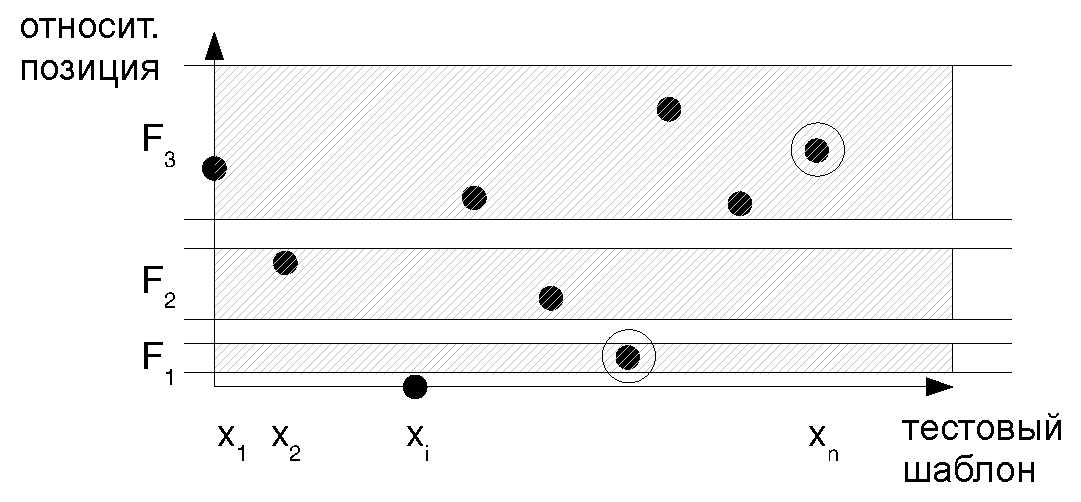
\includegraphics[width=0.8\textwidth]{2.theor/plru-feeds-useful}\\
%  \caption{К доказательству леммы~\ref{lemma_plru_hit''}}\label{plru-feeds-useful}
%\end{figure}
%
%  Покажем, что $c$ есть количество черных вершин в ветви к моменту
%  после $x_n$. Справедливо условие $u_i \in
%  [\frac{w}{2^k},~\frac{w}{2^{k-1}})$, где $k = F(u_i)$.
%  Следовательно, по теореме~\ref{thm_pseudoLRU_invariant} $u_i$
%  красит в черный цвет $W-k+1$'й элемент ветви, а $1, 2,..., W-k$'е
%  -- в белый. Так как после $u_i$ не будет больше инструкций,
%  перекрашивающих $W{-}k{+}1$'й элемент ветви в черный цвет (по
%  построению $u_i$), то $u_i$ является последним тегом, который
%  красит в черный цвет $W-k+1$'й элемент ветви. Пусть среди
%  $u_1,~u_2,~\dots,~u_c$ отсутствует представитель какой-нибудь
%  полосы, например, $k$'й. Тогда всегда существует представитель
%  более нижней полосы (поскольку для первой полосы всегда имеется
%  представитель в полезной последовательности). Это означает, что
%  этот более нижний представитель красит $W{-}k{+}1$'й элемент ветви
%  в белый цвет и никакие другие инструкции не могут перекрасить этот
%  элемент в черный цвет. Таким образом, показано взаимнооднозначное
%  соответствие наличия в полезной последовательности представителя
%  полосы и цвет соответствующего элемента ветви (черный в случае
%  наличия представителя). Из этого будет следовать, что $c$ и есть
%  количество черных вершин в ветви.
%
%  Значит, при $c < W$ тег не будет вытеснен, поскольку его ветвь
%  будет содержать хотя бы один белый элемент. $c$ есть количество
%  тегов тестового шаблона $x_i$, входящих в полезную
%  подпоследовательность. Т.е. количество $x_i$, для которых
%  выполняется критерий попадания в полезную подпоследовательность.
%  Обозначим этот критерий $u(x_i)$. Он равен 1 тогда и только тогда,
%  когда $x_i$ есть в полезной последовательности. Получаем, что $c =
%  \sum u(x_i)$. Осталось показать, что этот критерий -- и есть
%  предложенная в формулировке теоремы функция полезности.
%
%  Действительно, если тег $x_i$ попал в полезную последовательность,
%  то по определению следующие за ним теги будут лежать в более
%  высоких полосах. Т.е. для всех $j > i$ ($j \leqslant n$)
%  $F(\delta_j) > F(\delta_i)$, где $\delta_j$ и $\delta_i$ --
%  относительные позиции тегов $x_j$ и $x_i$. Условие сравнения $F$
%  будет выполнено в том и только в том случае, когда множества
%  $[2^{W-k_i},~2^{W-k_i+1})$ и
%  $[2^{W-k_j},~2^{W-k_j+1})$, где $k_i = F(x_i)$,
%  $k_j = F(x_j)$, не пересекаются. Т.е. существует такой $k$, что
%  $\delta_i < 2^k \leqslant \delta_j$, что и есть по определению $P(\delta_i,
%  \delta_j)$.
%
%  Осталось показать, что $P(x,y)$ выполнено тогда и только тогда
%  (т.е. что существует такой $k$, что $x < 2^k \leqslant y$, тогда и
%  только тогда), когда $(y > x \wedge y
%  \oplus x > x)$, где $0\leqslant x, y < w$. Действительно, если
%  выполнена левая часть, то количество старших нулей в $y$ меньше
%  количества старших нулей в $x$. Следовательно, в сумме по модулю 2
%  $y$ и $x$ количество старших нулей будет равно минимуму количеств
%  старших нулей в $y$ и $x$, т.е. то, каково оно в $y$. Но поскольку
%  оно меньше, чем в $x$, то $y \oplus x > x$. А $y > x$
%  непосредственно следует из $x < 2^k \leqslant y$. В обратную
%  сторону. Пусть количество старших нулей в $y$ больше или равно
%  количеству старших нулей в $x$. Если оно больше, то значения $x$ и
%  $y$ разделяет число (0 0... 0 1 0 ....0), в котором количество
%  старших нулей равно количеству старших нулей в $x$. Тем самым $y <
%  x$. Если же количества старших нулей в $x$ и $y$ совпадают, то в
%  $x \oplus y$ будет как минимум на 1 больше старших нулевых бит,
%  поскольку старшие единицы в $x$ и $y$ в сумме дали 0.
%  Эквивалентность доказана.
%
%  Кроме того, в критерий $u(x_i)$ надо добавить условие совпадения
%  регионов $R(x) = R(x_i)$, поскольку вытеснение определяется только
%  для тегов одного региона, и условие случившегося последнего
%  обращения к $x$, что выражается формулой $x \notin \{x_i, x_{i+1},
%  ..., x_{m-1}\}$.
%
%  Все эти рассуждения велись с целью описания свойства ветви после
%  $x_n$. Значит, оно справедливо и для тех $x_m$, которые дают
%  кэш-промах. Если хотя бы перед одним из них ветвь станет полностью
%  черной, то тег $x$ будет вытеснен. Значит, чтобы он не был
%  вытеснен, надо чтобы для всех $x_m$, дающих кэш-промах,
%  $\sum_{i=1}^{m-1} u_m(x_i) < W$.
%\end{proof}
%
%\begin{lemma}\label{lemma_plru_hit'}
%Пусть $x$ -- тегсет текущей инструкции при стратегии вытеснения
%\PseudoLRU. Тогда если $x = \lambda \in L_0$ и $x \notin \{x_1, x_2,
%..., x_n\}$, где $x_1, x_2, ..., x_n$ -- тегсеты предыдущих
%инструкций, то $x$ не вытеснен к моменту текущей инструкции согласно
%каноническому определению \PseudoLRU тогда и только тогда, когда для
%каждого $x_m$ : miss ($1 \leqslant m \leqslant n$) выполнено
%$\sum_{i=1,...,W:\xi_i = 1} v_m(\xi_i) + \sum^{m-1}_{i=1} u_m(x_i) <
%W$, где $W = \log_2 w$, $(\xi_1~\xi_2~\dots~\xi_W)$ -- начальные
%цвета ветви, ведущей в $\lambda$, а $u_m(x_i)$ (\emph{функция
%полезности}) определена следующим образом:
%$$u_m(x_i) \equiv
%    (R(x_i) = R(x) \wedge \bigwedge_{j=i+1}^{m-1} P(\pi_i \oplus \pi,
%       \pi_j \oplus \pi))$$
%$$P(\delta_i, \delta_j) \equiv (\delta_j > \delta_i~~\wedge~~\delta_j \oplus \delta_i > \delta_i)$$
%$$v_m(\xi_i) \equiv
%    \bigwedge_{j=1}^{m-1} P(2^{W-i} \oplus \pi, \pi_j \oplus \pi)$$
%\end{lemma}
%\begin{proof}
%  Проводится аналогично доказательству леммы~\ref{lemma_plru_hit''}.
%  Начальное состояние ветви моделируется <<псевдотегами>>
%  $\xi_1,~\xi_2,~\dots,~\xi_W$. Их относительные позиции равны
%  соответственно $(1 0 ...0), (0 1 0 .... 0), ..., (0 .... 0 1)$,
%  т.е. $2^{W-1},~2^{W-2},~\dots,~1$.
%\end{proof}
%
%\begin{theorem}[корректность использования функций полезности для
%записи \PseudoLRU] Тестовая программа, построенная по ограничениям,
%которые сгенерированы с использованием предъявленных выше функций
%полезности, удовлетворяет своему тестовому шаблону.
%\end{theorem}
%\begin{proof}
%  Доказывается аналогично доказательству
%  теоремы~\ref{thm_lru_usefulness_correct} c использованием
%  доказанных ранее лемм. Для случаев кэш-промаха леммы формулируются
%  как обратные к леммам про кэш-попадание, что обосновывает их
%  истинность.
%\end{proof}
%
%
%\section*{Корректность использования функций полезности для
%записи \LRU в специальных тестовых шаблонах}
%
%\begin{theorem}[корректность использования функций полезности для
%записи \LRU в коротких тестовых шаблонах]\label{short_templates}
%Тестовая программа, построенная по ограничениям, которые
%сгенерированы с использованием предъявленных в
%таблице~\ref{short_templates_table} функций полезности,
%удовлетворяет своему короткому тестовому шаблону.
%\end{theorem}
%\begin{proof}
%  Для короткого шаблона, как и для любого другого, справедлива
%  теорема~\ref{thm_lru_usefulness_correct} и
%  таблица~\ref{hit_miss_table}. Однако не все выделенные в них
%  ситуации в коротких шаблонах возможны. Поскольку в коротком
%  шаблоне не может быть более $w$ инструкций обращения к памяти, то
%  и количество полезных инструкций не может быть более $w$. Значит,
%  подформулы $\sum u(x_i) \geqslant w$ являются тождественно
%  ложными, а подформулы $\sum u(x_i) < w$ --- тождественно
%  истинными. Таким образом, пятая и седьмая строчки
%  таблицы~\ref{hit_miss_table} не попадут в таблицу для коротких
%  шаблонов, а из второй и третьей строчек нужно исключить
%  неравенство с суммой функций полезности (в этих строчках функции
%  полезности не нужны вовсе).
%
%  Дизъюнкция получившихся первых трех строк системы выглядит следующим образом:
%  $$\left[\begin{array}{l}
%        \left\{\begin{array}{l}
%            x = \lambda_\delta\\
%            x \notin \{x_1,~x_2,~\dots,~x_n\}\\
%            \sum_{i=1}^n u(x_i) \leqslant w - \delta\\
%        \end{array}\right.\\[1cm]
%        \left\{\begin{array}{l}
%            x = \lambda_\delta\\
%            x \in \{x_1,~x_2,~\dots,~x_n\}\\
%        \end{array}\right.\\
%        x \in [x_1,~x_2,~\dots,~x_n]_{\mbox{miss}}\\
%    \end{array}\right.$$
%    что эквивалентно следующей системе:
%  $$\left[\begin{array}{l}
%        \left\{\begin{array}{l}
%            x = \lambda_\delta\\
%            \sum_{i=1}^n u(x_i) \leqslant w - \delta\\
%        \end{array}\right.\\[1cm]
%        \left\{\begin{array}{l}
%            x = \lambda_\delta\\
%            x \in \{x_1,~x_2,~\dots,~x_n\}\\
%        \end{array}\right.\\
%        x \in [x_1,~x_2,~\dots,~x_n]_{\mbox{miss}}\\
%    \end{array}\right.$$
%
%    Покажем, что справедливо следующее эквивалентное преобразование:
%  $$\left[\begin{array}{l}
%        \left\{\begin{array}{l}
%            x = \lambda_\delta\\
%            x \in \{x_1,~x_2,~\dots,~x_n\}\\
%        \end{array}\right.\\
%        x \in [x_1,~x_2,~\dots,~x_n]_{\mbox{miss}}\\
%    \end{array}\right. \Leftrightarrow x \in \{x_1,~x_2,~\dots,~x_n\}$$
%
%    Обозначим, $\alpha \equiv (x = \lambda_\delta)$, $\beta \equiv (x \in
%    [x_1,~x_2,~\dots,~x_n]_{\mbox{hit}})$, $\gamma \equiv (x \in
%    [x_1,~x_2,~\dots,~x_n]_{\mbox{miss}})$. Тогда надо доказать
%    следующую эквивалентность: $\alpha (\beta \vee \gamma) \vee \gamma \equiv
%    \beta \vee \gamma$. Для начала упростим ее с помощью
%    эквивалентных преобразований: $\alpha (\beta \vee \gamma) \vee \gamma \equiv
%    \beta \vee \gamma \Leftrightarrow \alpha \beta \vee \gamma \equiv
%    \beta \vee \gamma \Leftrightarrow (\alpha \beta \vee \gamma)(\beta \vee \gamma)
%    \vee \neg(\alpha \beta \vee \gamma)\neg(\beta \vee \gamma)
%    \Leftrightarrow (\alpha \beta \vee \gamma) \vee (\neg \alpha
%    \vee \neg \beta)\neg \gamma \neg \beta \Leftrightarrow (\alpha \beta \vee \gamma) \vee
%    \neg \gamma \neg \beta \Leftrightarrow \alpha \vee \gamma \vee \neg \beta$.
%
%    Итак, эквивалентность будет показана, если будет доказано, что:
%  $$\left[\begin{array}{l}
%        x = \lambda_\delta\\
%        x \in [x_1,~x_2,~\dots,~x_n]_{\mbox{miss}}\\
%        x \notin [x_1,~x_2,~\dots,~x_n]_{\mbox{hit}}\\
%    \end{array}\right.$$
%
%    Из теоремы~\ref{thm_lru_usefulness_correct} следует, что $x \in L_0 \vee x \in
%    [x_1,~x_2,~\dots,~x_n]_{\mbox{miss}}$, из чего следует и
%    требуемая эквивалентность.
%
%    Таким образом, если при обращении к $x$ происходит
%    кэш-попадание, то для $x$ справедливы следующие условия:
%  $$\left[\begin{array}{l}
%        \left\{\begin{array}{l}
%            x = \lambda_\delta\\
%            \sum_{i=1}^n u(x_i) \leqslant w - \delta\\
%        \end{array}\right.\\[1cm]
%        x \in \{x_1,~x_2,~\dots,~x_n\}\\
%    \end{array}\right.$$
%\end{proof}
%
